\documentclass{beamer}

\usepackage[english, german]{babel}


\title{webchess}
\subtitle{Schach Plattform Web-App in Haskell}
\author{Maximilian Lutz}

%\usetheme{Madrid}
\usetheme[progressbar=frametitle]{metropolis}
\definecolor{carbonblack}{HTML}{151718}
\definecolor{carbonprogbar}{HTML}{E6CD69}
\setbeamercolor{frametitle}{bg=carbonblack}
\setbeamercolor{alerted text}{fg=carbonprogbar}
%\usecolortheme{seahorse}

\begin{document}



\maketitle

% DEMO

% \begin{frame}{Features}

% \centering
% \textbf{Web-Plattform f\"ur Schach}

% \begin{itemize}
%     \item Account System (Userpages, Authentifizierung, Elo)
%     \item Spiel human-human (inkl. Spectator mode)
%     \item Soziale Features: Highscore Ranking, Lobby to find players
%     \item AI Spiele
% \end{itemize}

% \end{frame}

\begin{frame}[plain,c]
\begin{center}
\Huge Quick demo!
\end{center}
\end{frame}

% Structure

% \section{Struktur}

% \begin{frame}{Struktur}
% \begin{figure}
% 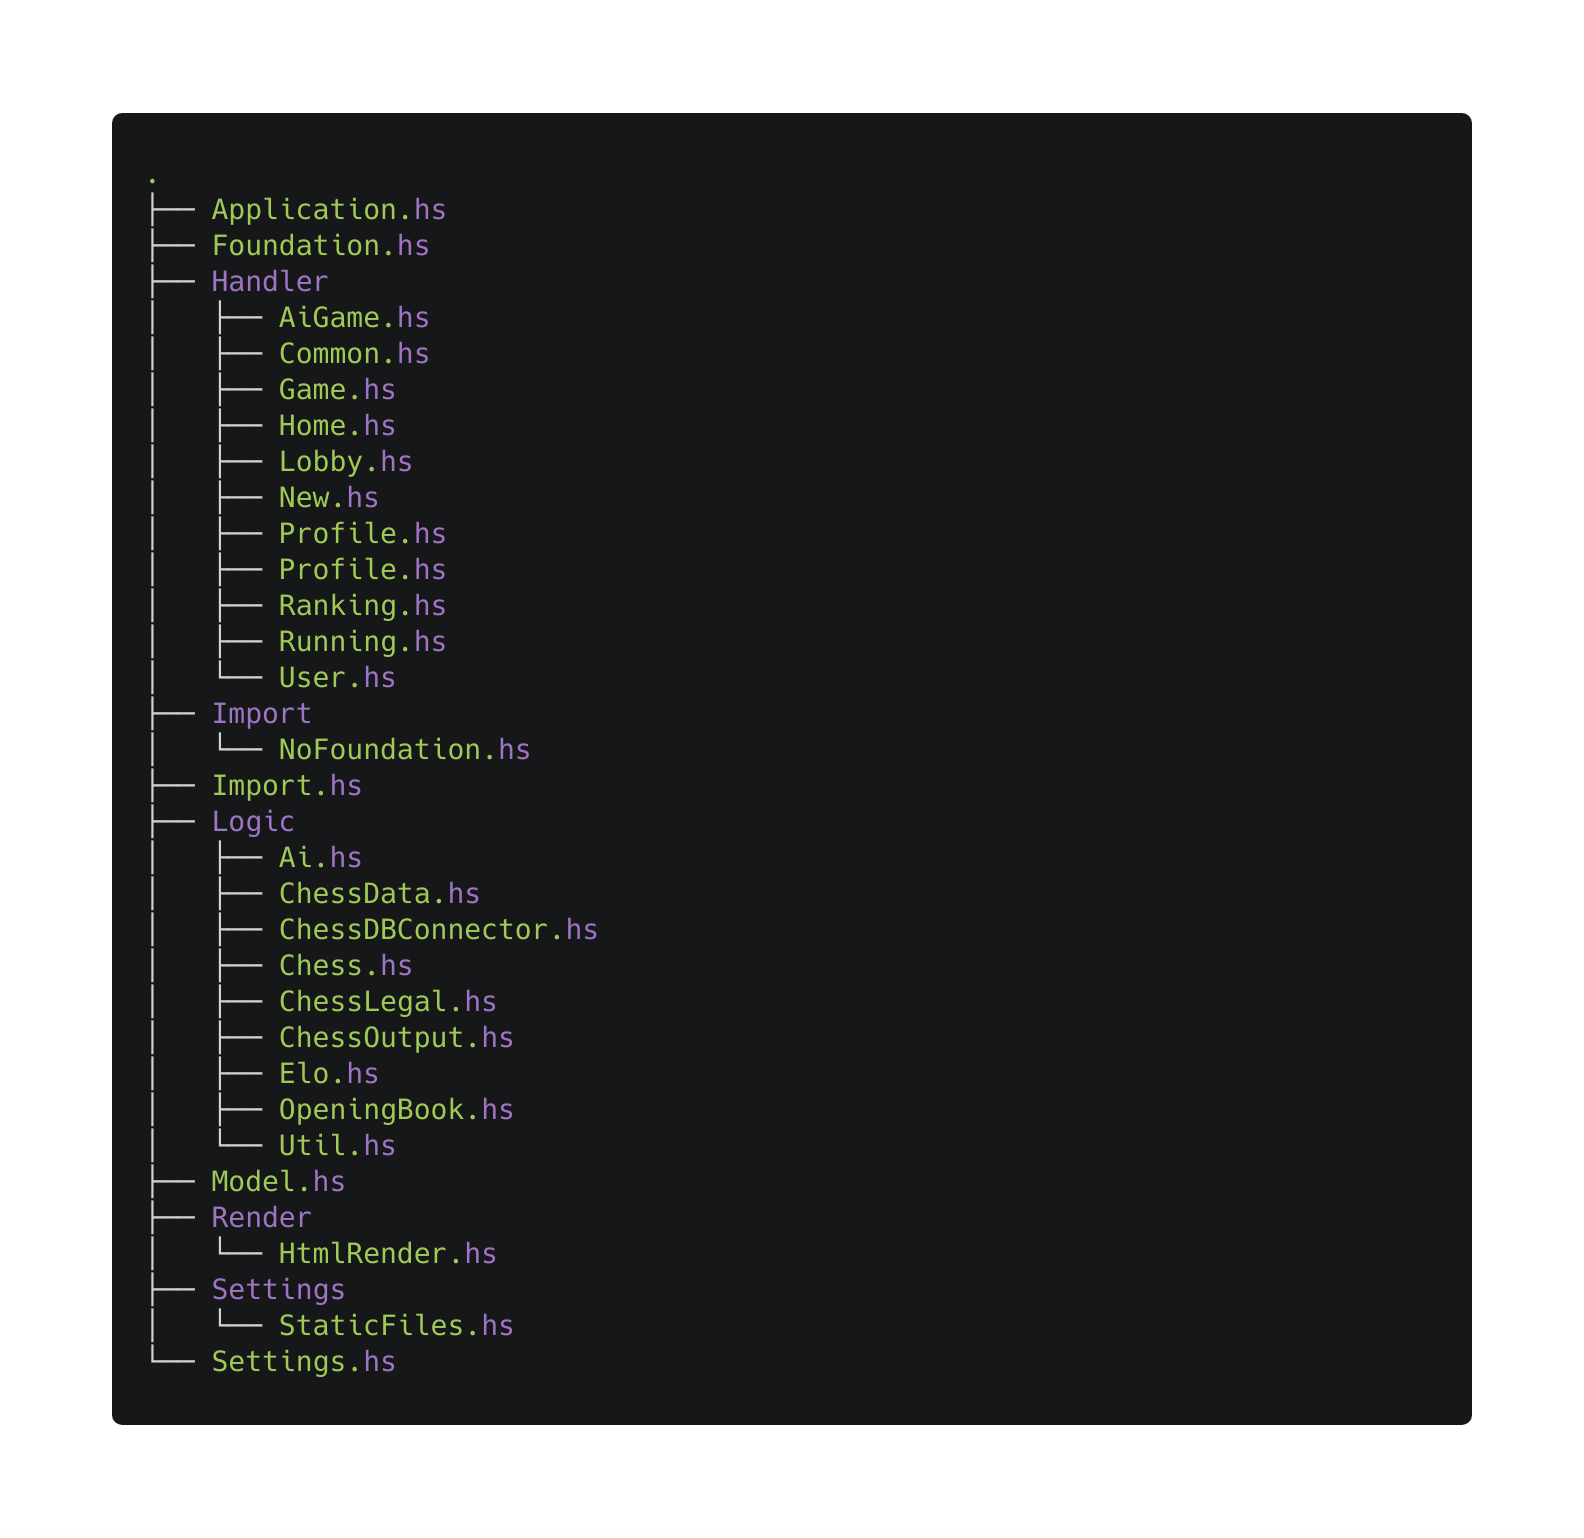
\includegraphics[height=\textheight]{tree1}
% \end{figure}
% \end{frame}

% \begin{frame}{Struktur}
% \begin{figure}
% 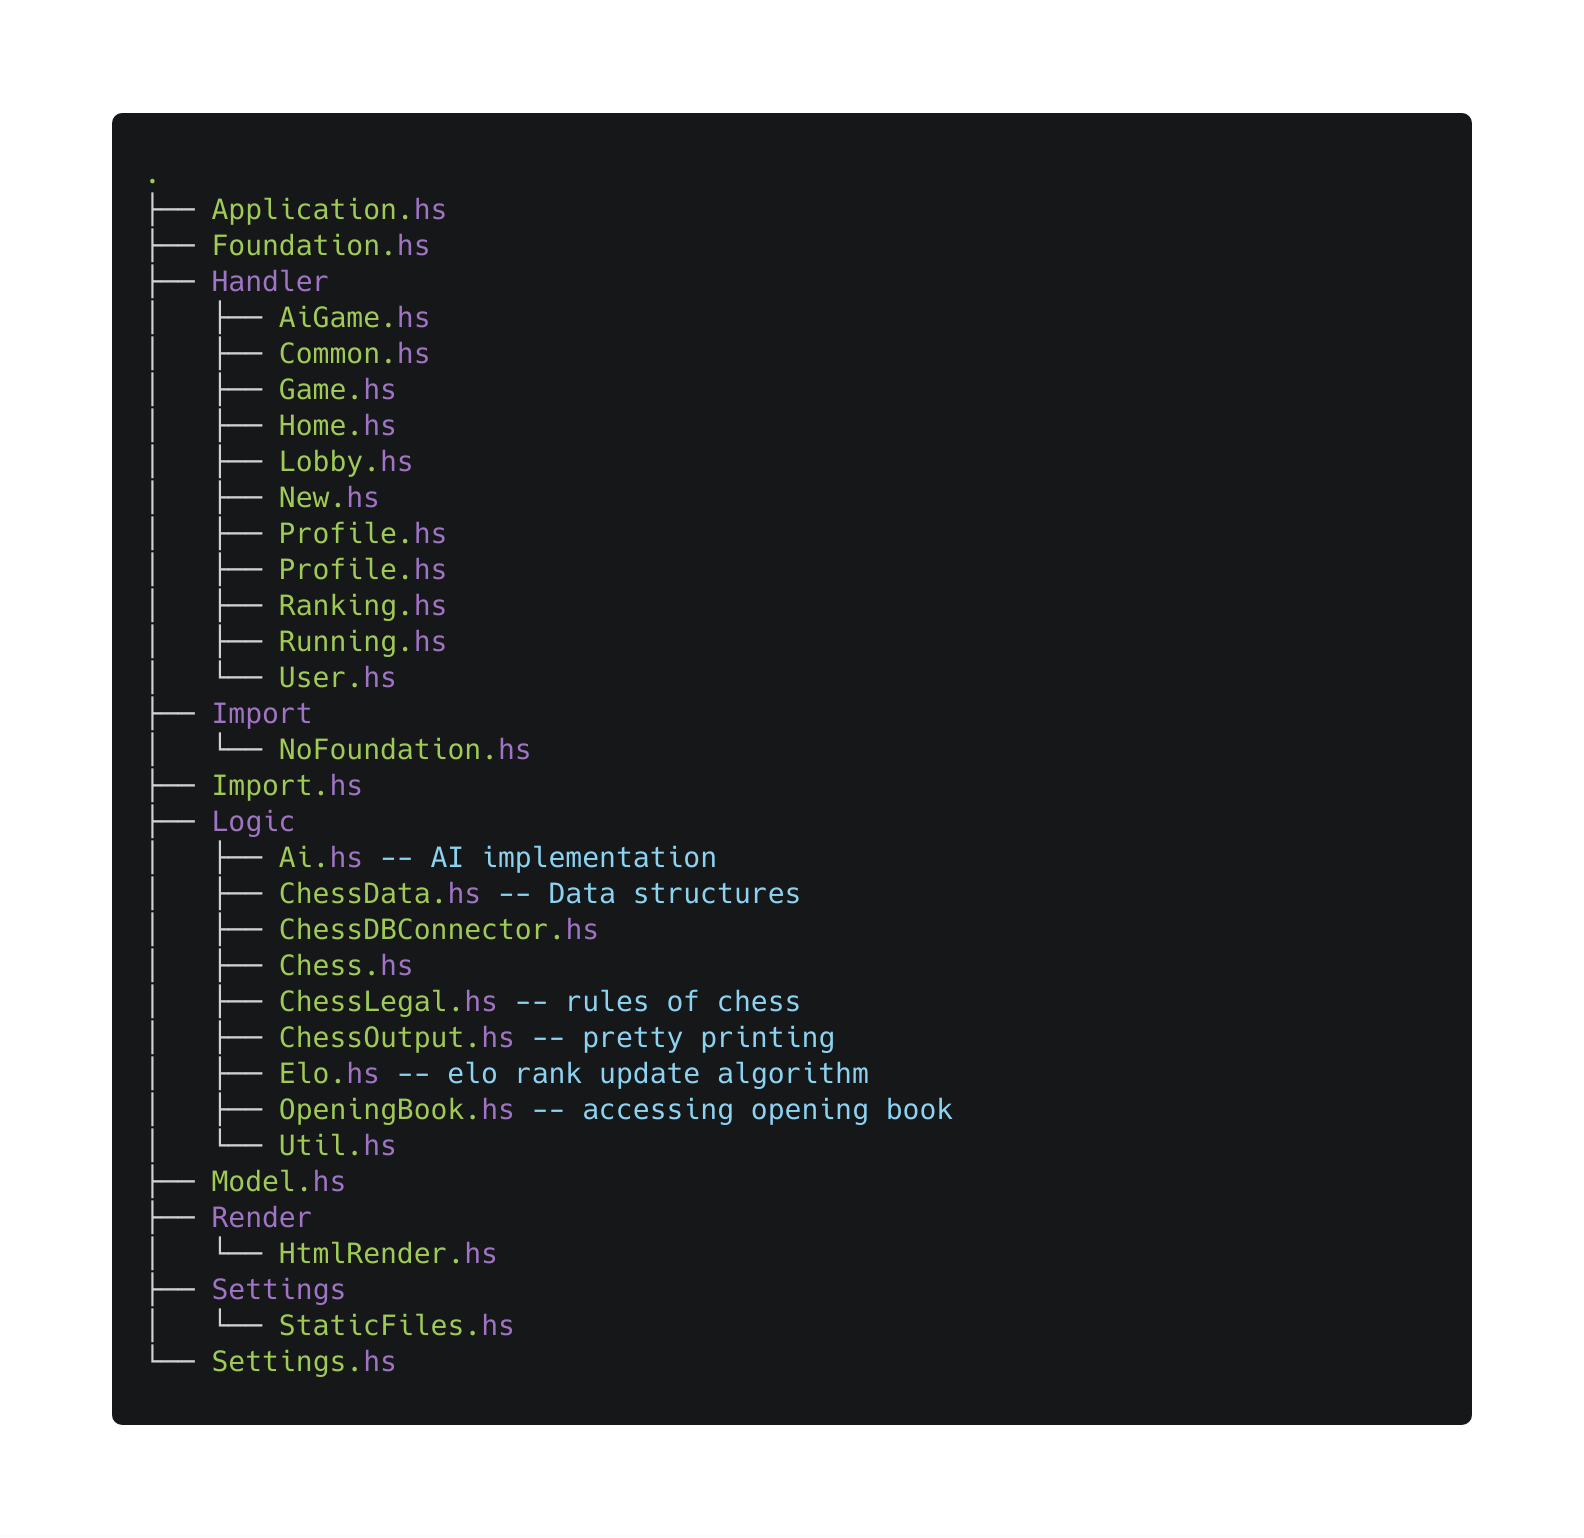
\includegraphics[height=\textheight]{tree2}
% \end{figure}
% \end{frame}

% \begin{frame}{Struktur}
% \begin{figure}
% 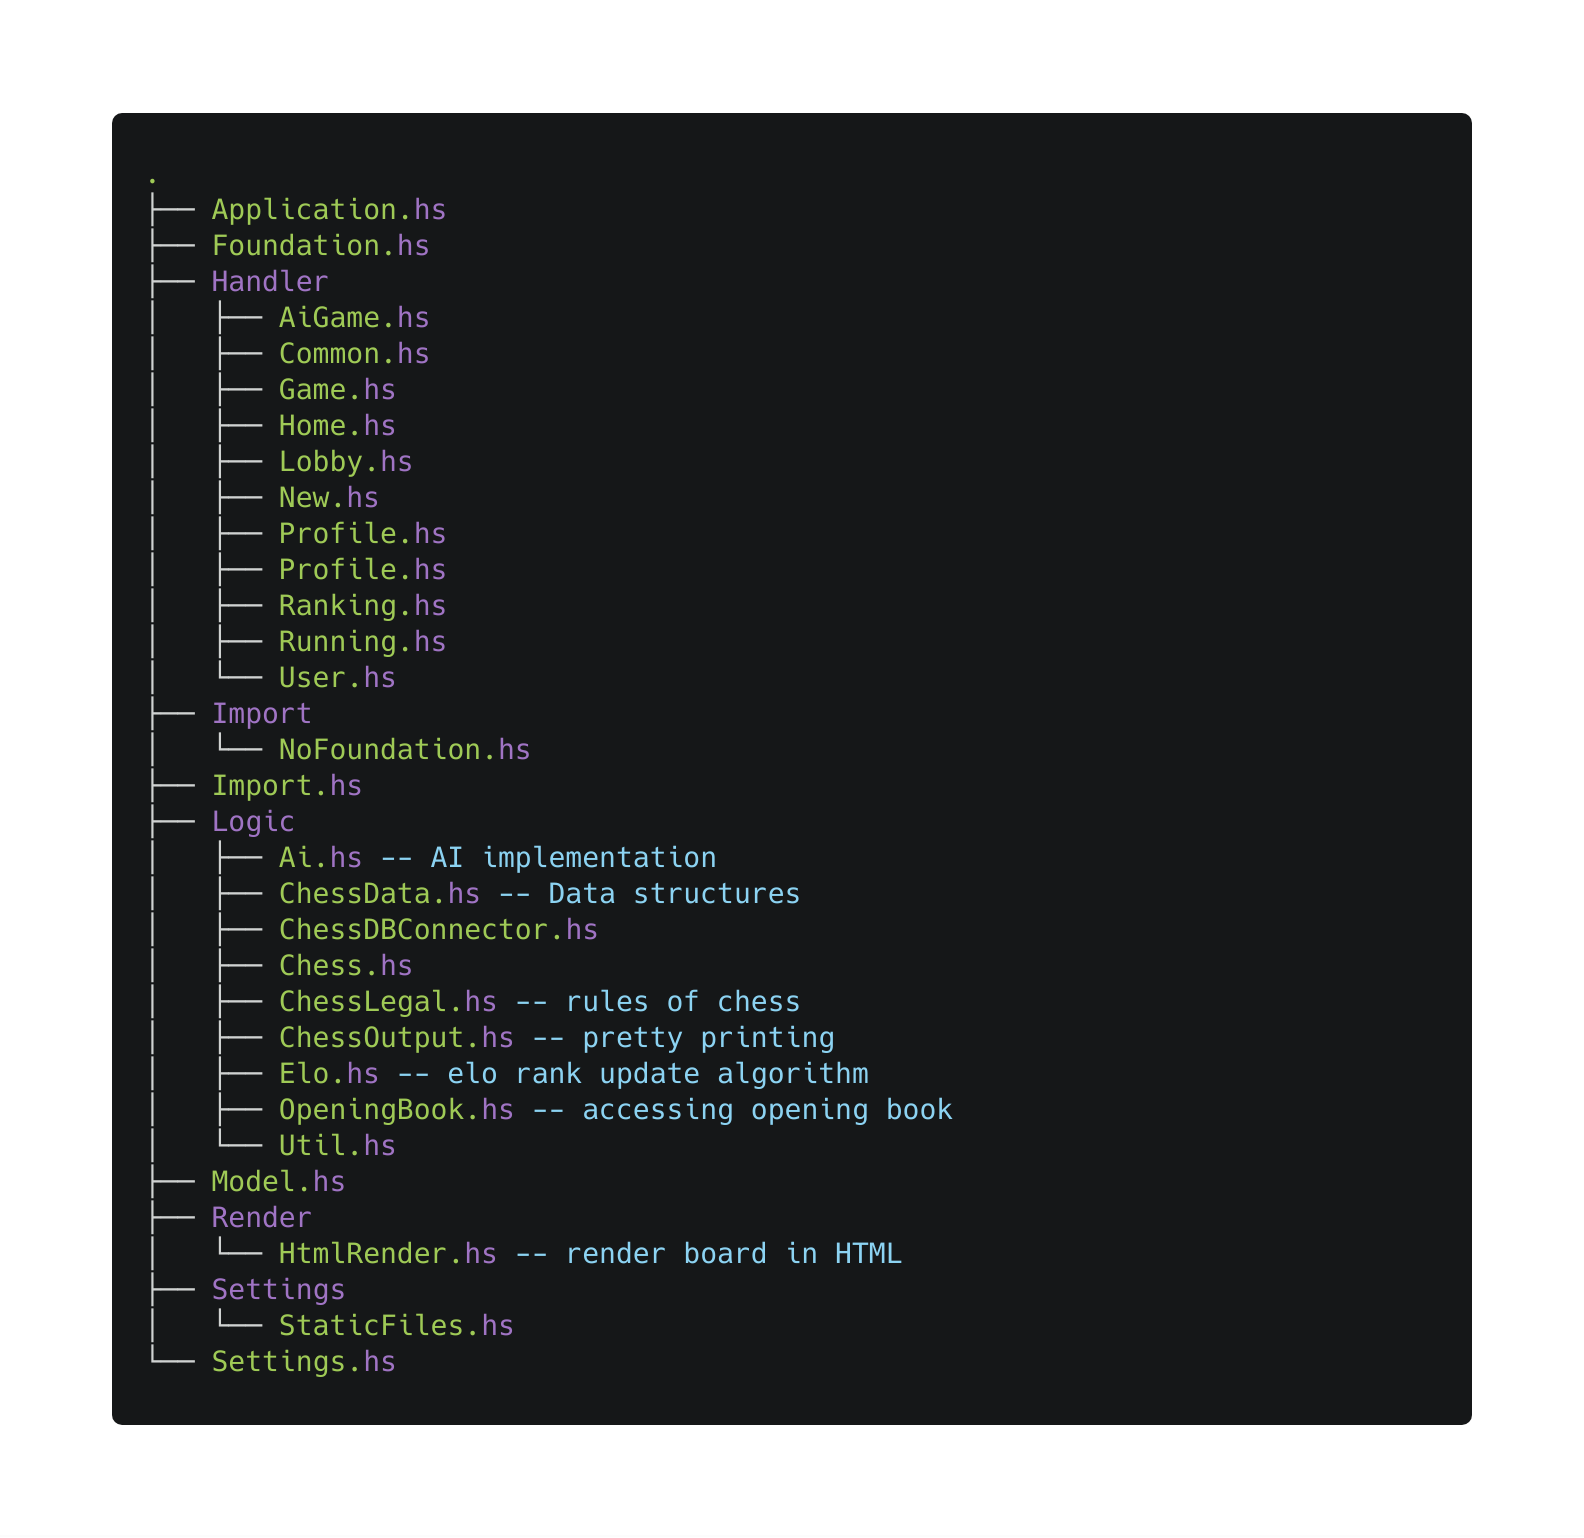
\includegraphics[height=\textheight]{tree3}
% \end{figure}
% \end{frame}

% \begin{frame}{Struktur}
% \begin{figure}
% 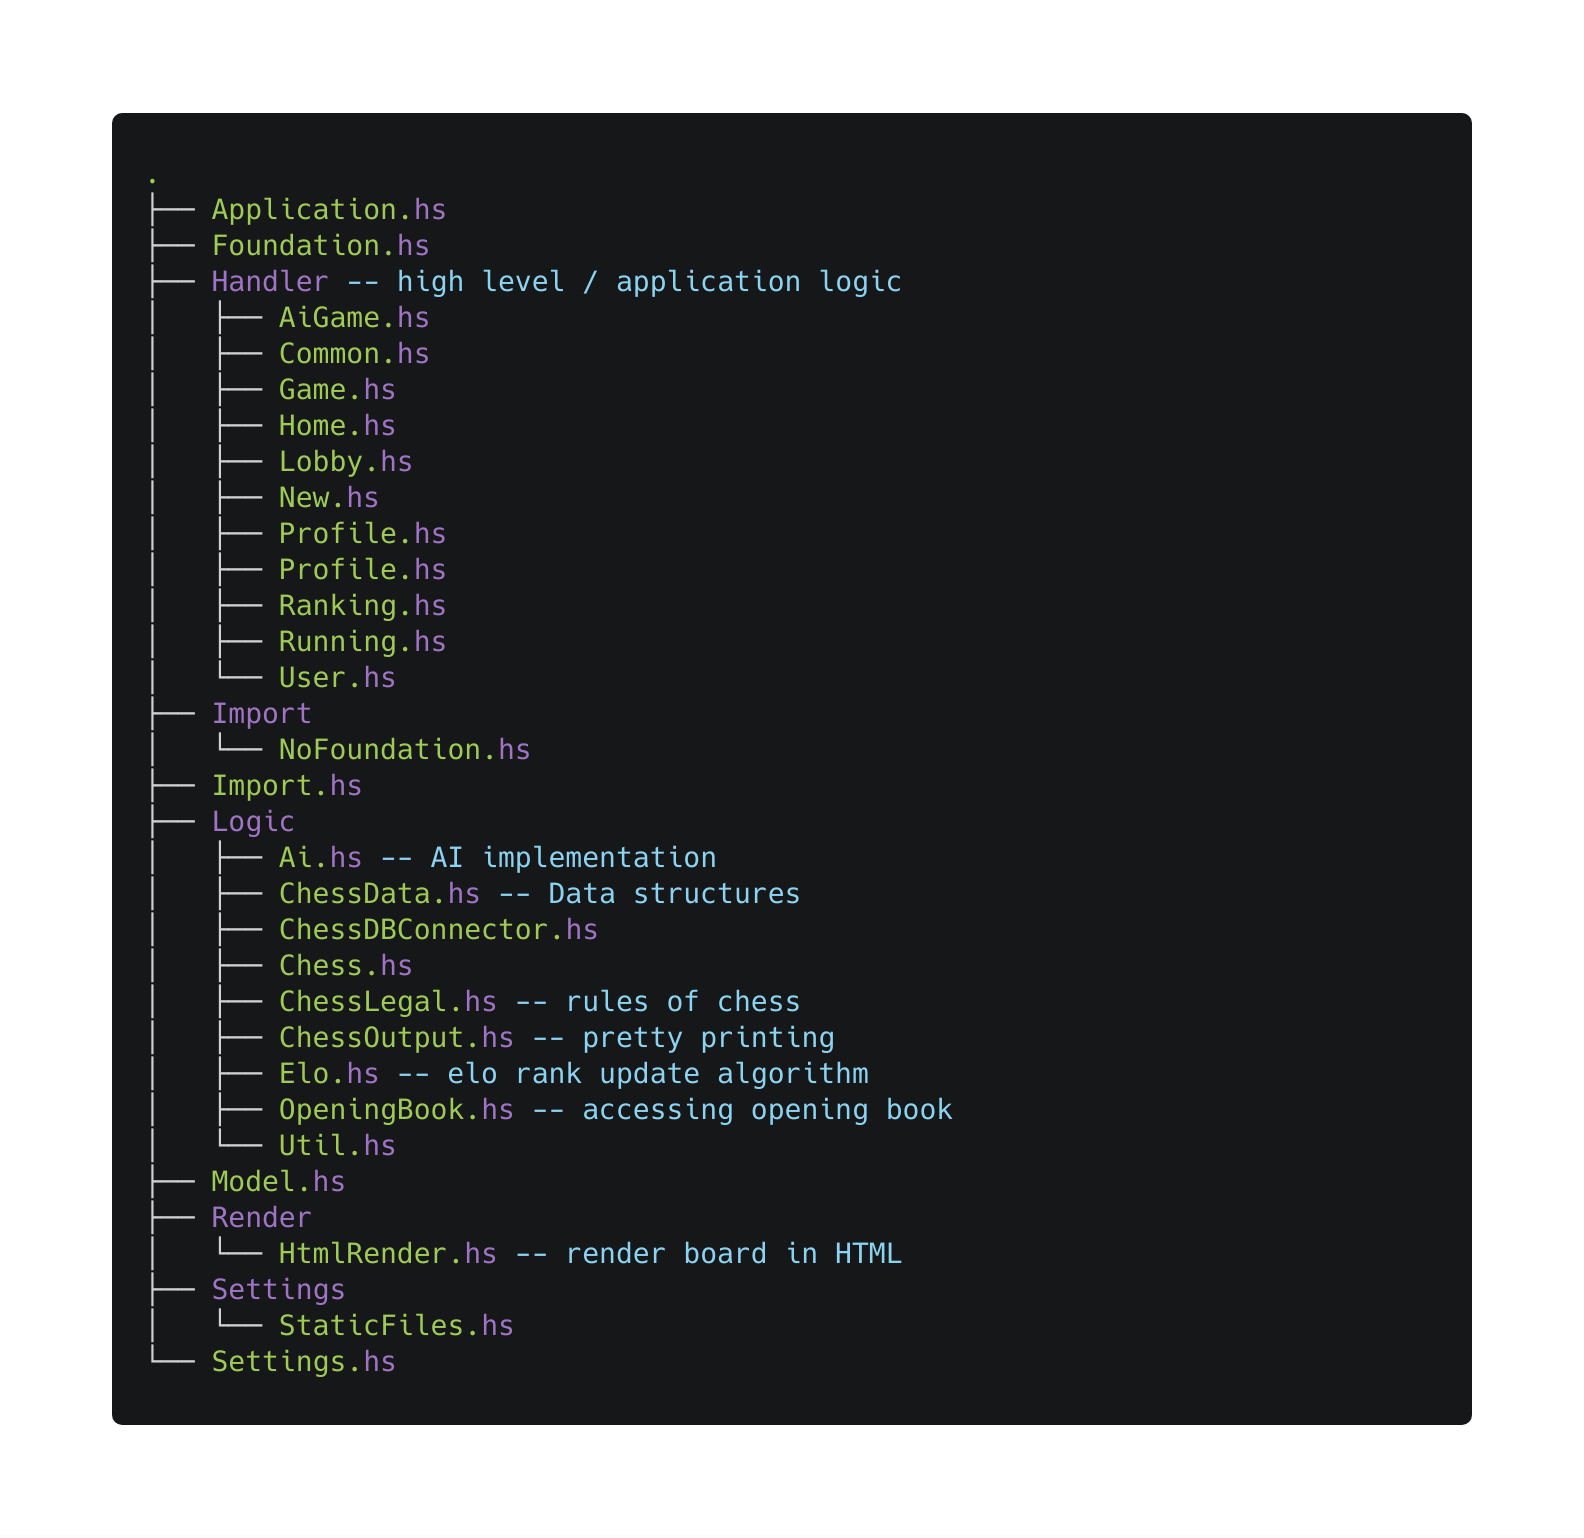
\includegraphics[height=\textheight]{tree4}
% \end{figure}
% \end{frame}

% Code

\section{Code \& Details}


\begin{frame}

\begin{columns}

\column{0.5\textwidth}
{\Large \textbf{Datenstruktur \& Spielregeln}}

\begin{itemize}
    \item Control.Lens
\end{itemize}

\column{0.5\textwidth}
\begin{figure}
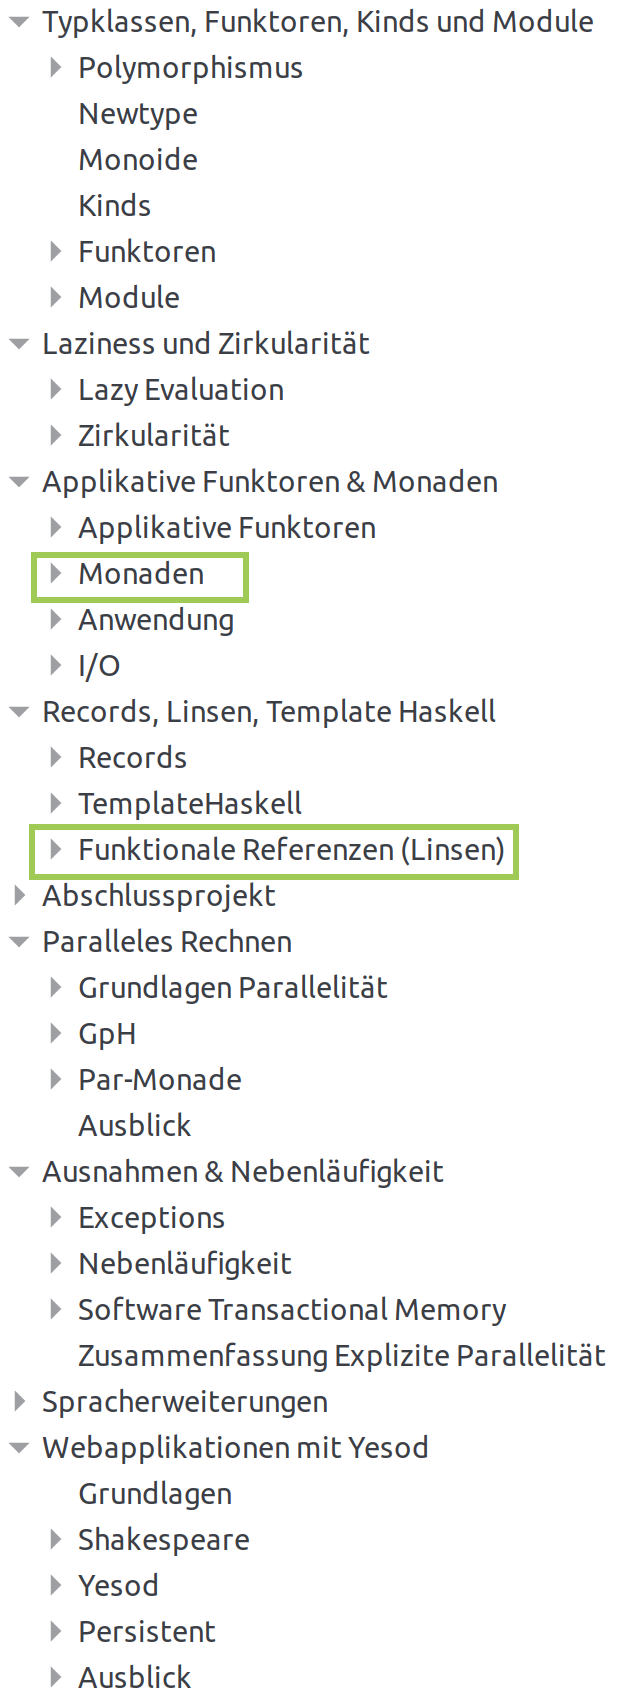
\includegraphics[height=0.9\paperheight]{cont/sschessdata.png}
\end{figure}

\end{columns}

\end{frame}



\begin{frame}{Datenstruktur}

\begin{figure}
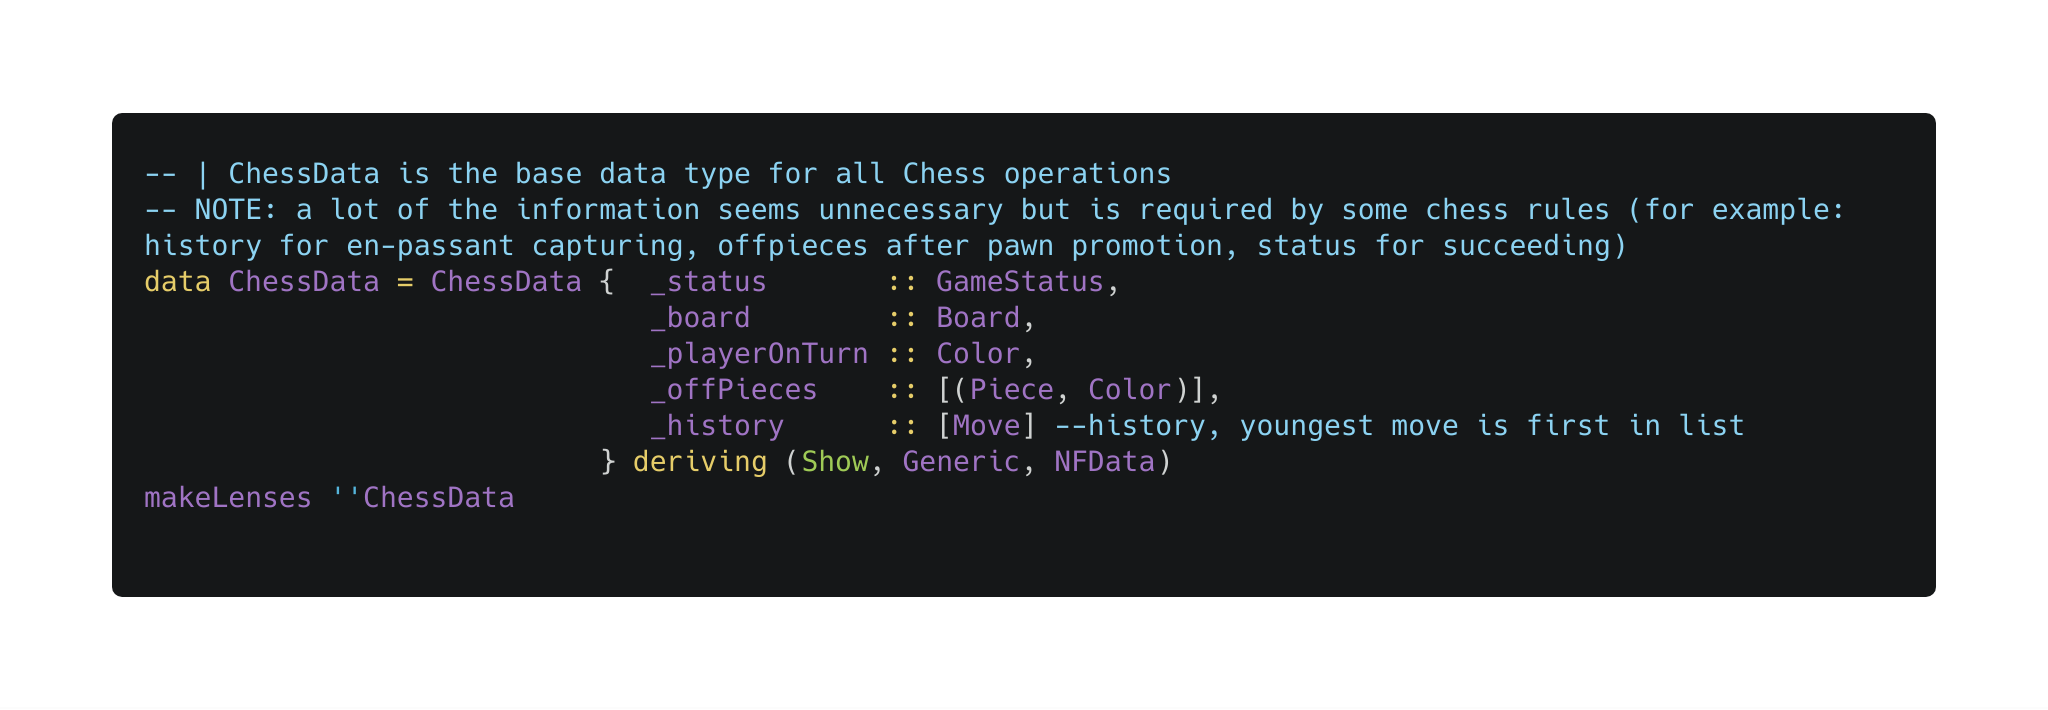
\includegraphics[width=\linewidth]{chessdata}
\end{figure}

\end{frame}

\begin{frame}{Spielregeln}

\begin{figure}
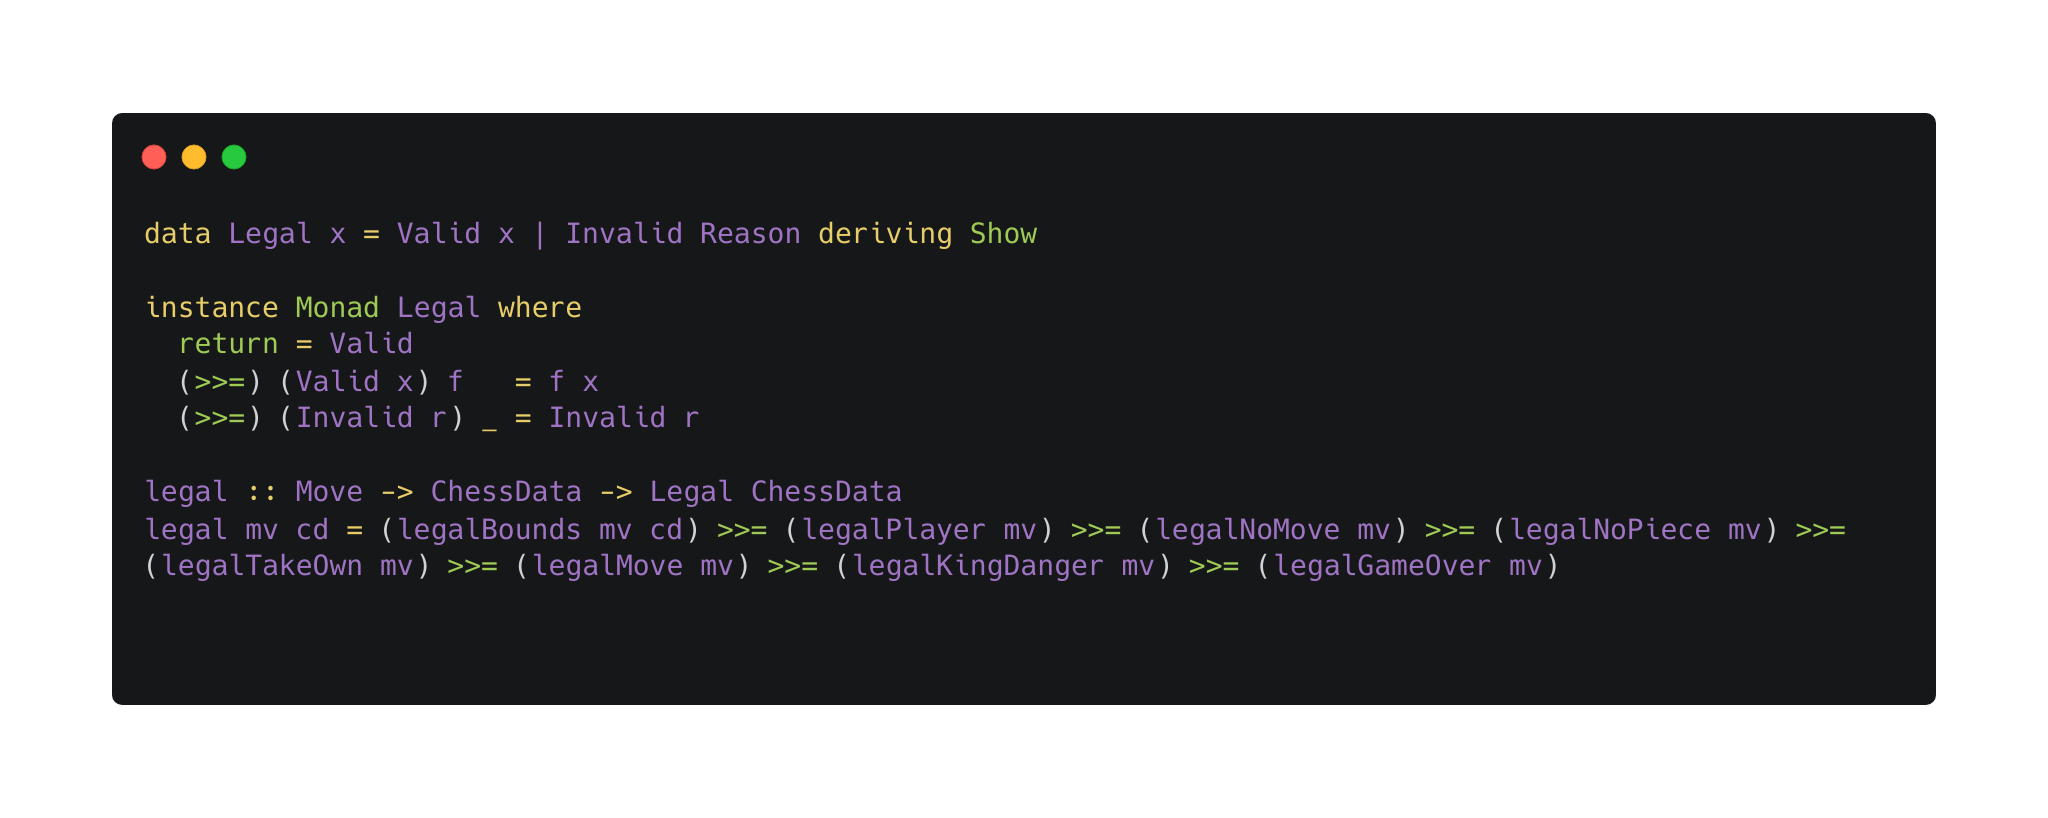
\includegraphics[width=\linewidth]{chesslegal}
\end{figure}

\end{frame}




\begin{frame}

\begin{columns}

\column{0.5\textwidth}
{\Large \textbf{AI}}

\begin{itemize}
    \item Control.Parallel.Strategies
    \item Data.Graph.Inductive
    \item insb. Inductive.PatriciaTree

\end{itemize}

\column{0.5\textwidth}
\begin{figure}
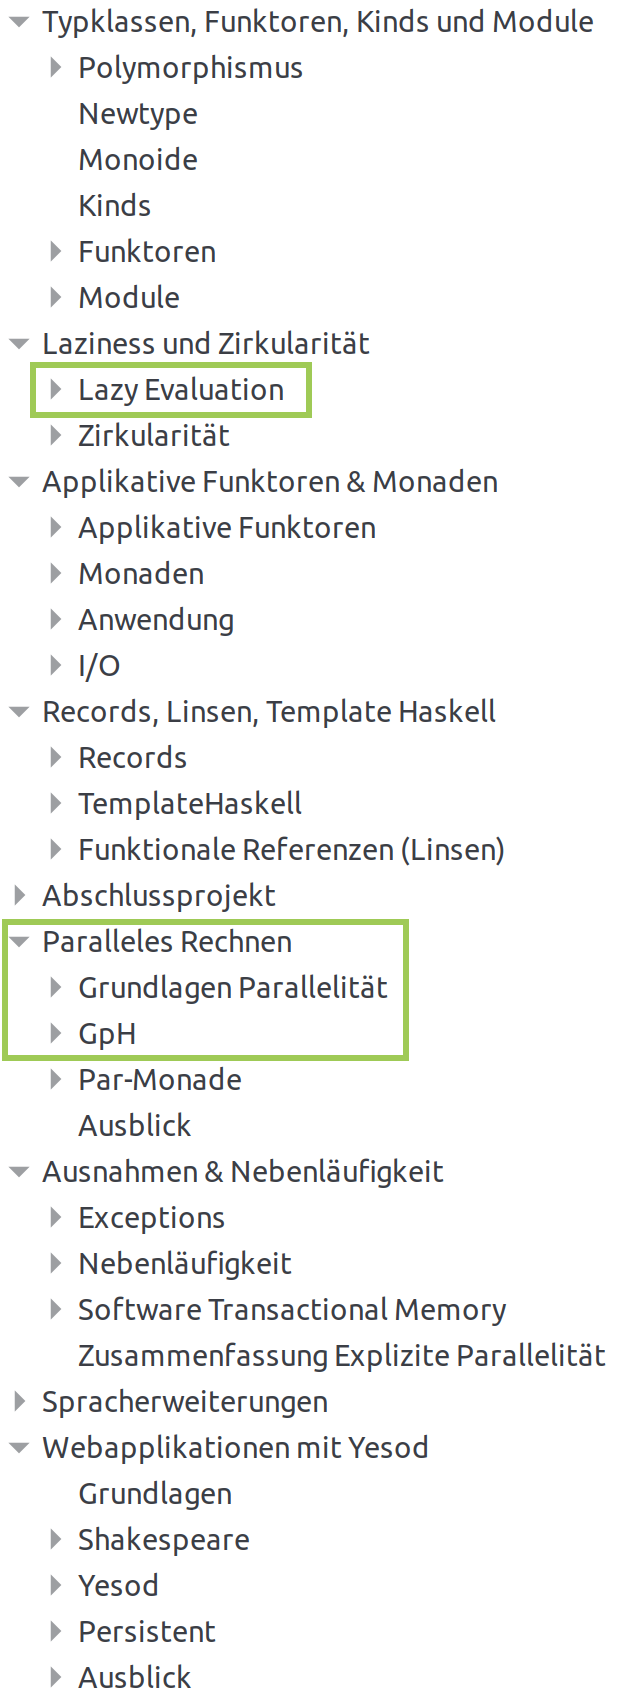
\includegraphics[height=0.9\paperheight]{cont/ssai.png}
\end{figure}

\end{columns}

\end{frame}

\begin{frame}{AI}
\begin{figure}
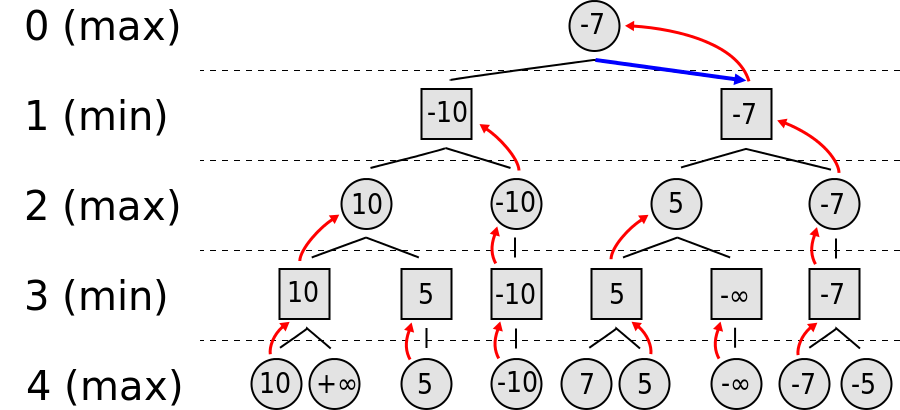
\includegraphics[width=\linewidth]{minmaxwiki.png}
%\caption{Visualisierung Min-Max Algorithmus}
\footnote{\tiny Von Nuno Nogueira (Nmnogueira) - http://en.wikipedia.org/wiki/Image:Minimax.svg, created in Inkscape by author, \textbf{CC BY-SA 2.5}, https://commons.wikimedia.org/w/index.php?curid=2276653}
\end{figure}
\end{frame}

\begin{frame}{AI}
\begin{figure}
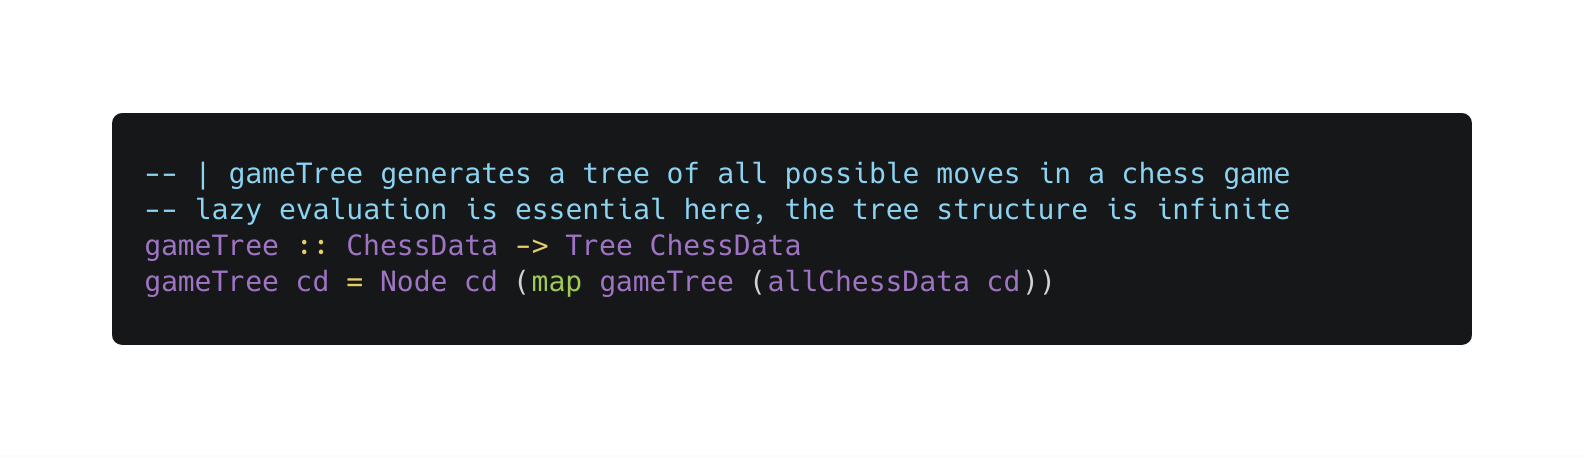
\includegraphics[width=\linewidth]{gametree}
\end{figure}
\end{frame}

\begin{frame}{AI}
\begin{figure}
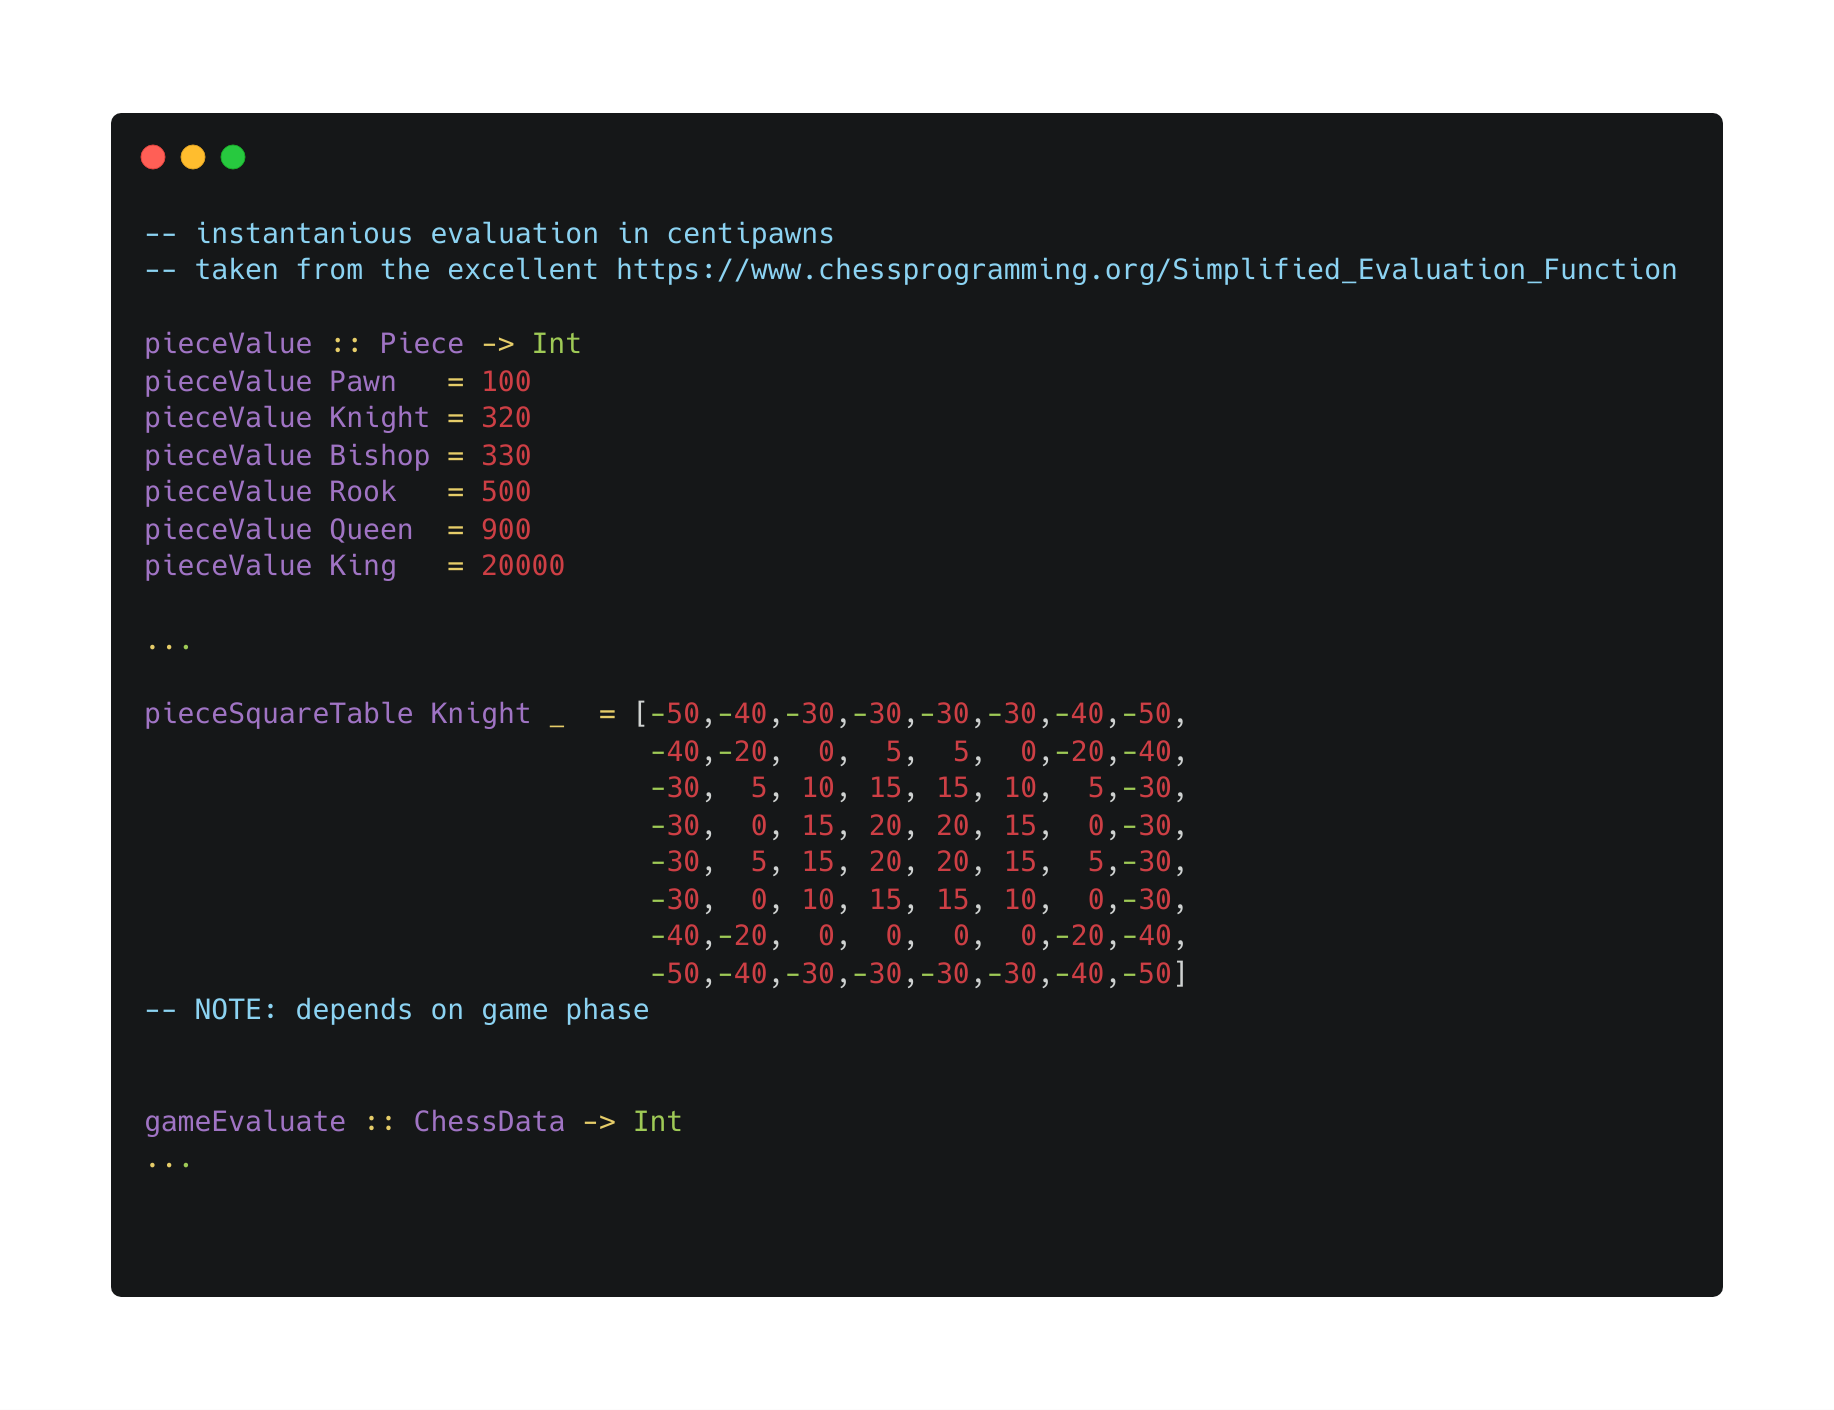
\includegraphics[width=\linewidth]{instanteval}
\end{figure}
\end{frame}

\begin{frame}{AI}
\begin{figure}
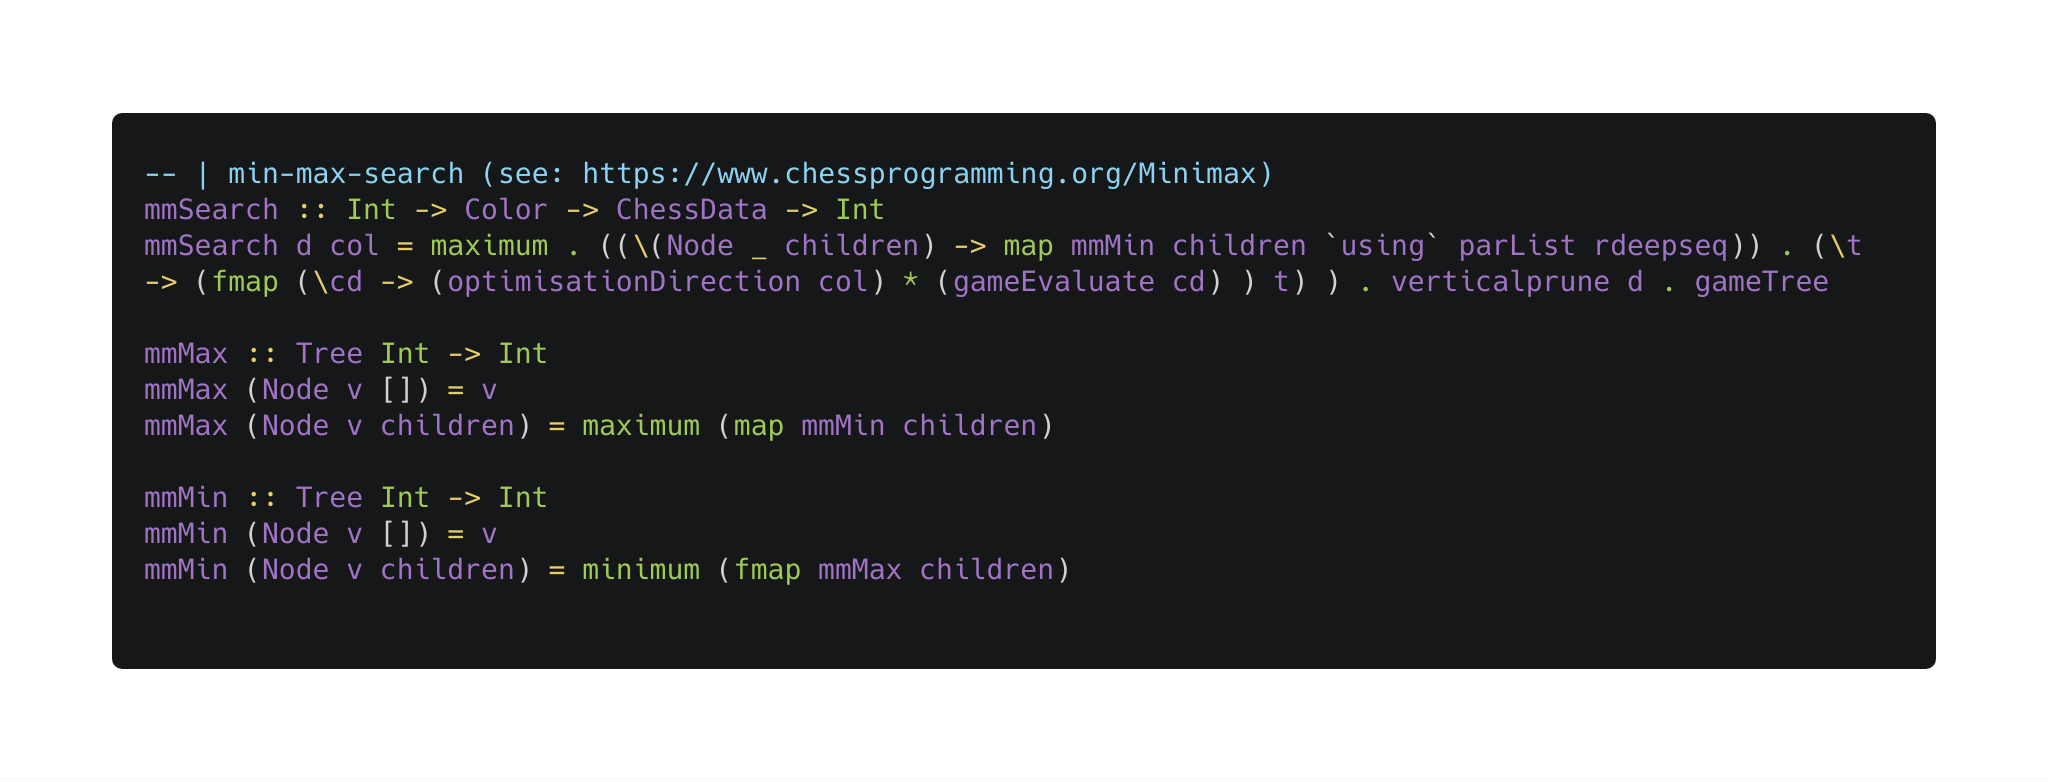
\includegraphics[width=\linewidth]{parminmax.png}
\end{figure}
\end{frame}

\begin{frame}{Threadscope}

\begin{figure}
   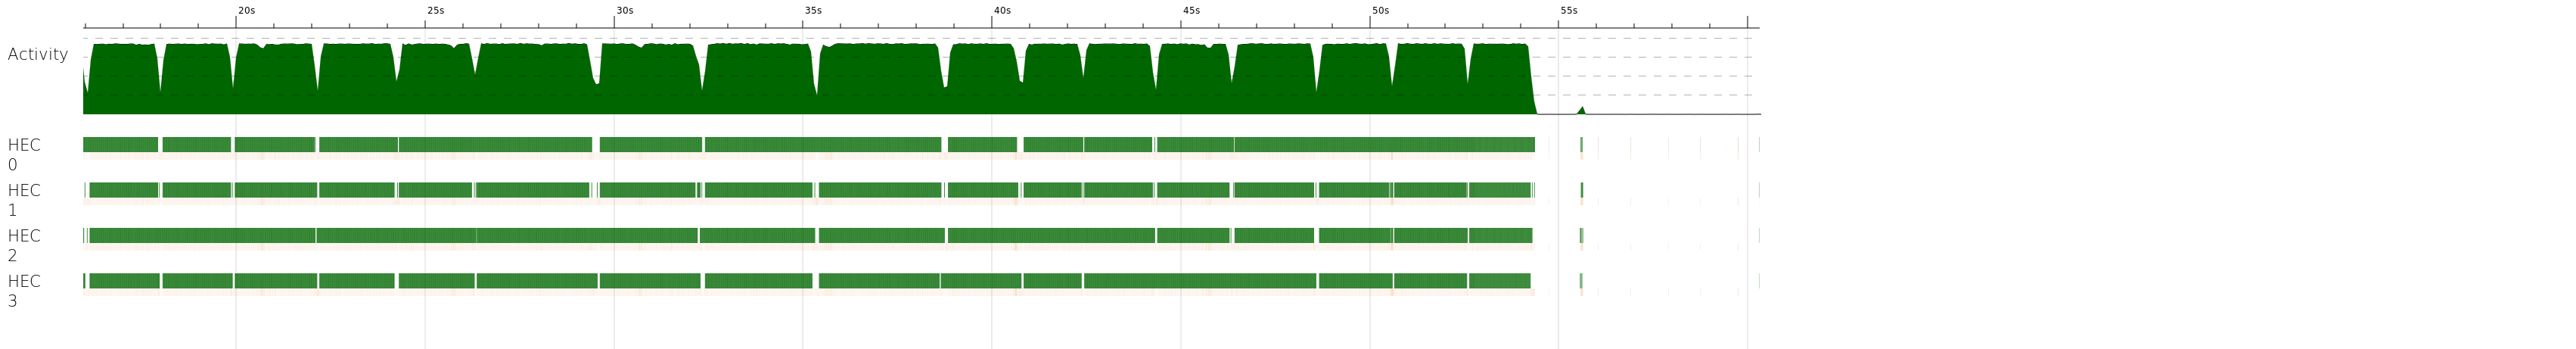
\includegraphics[width=1.5\linewidth]{4cores_zoom}
\end{figure}

Von 155.55s $\rightarrow$ 43.65s f{\"u}r -N1 Kern $\rightarrow$ -N4 Kerne ($\sim$ 3.6 speedup)
\end{frame}

\begin{frame}{AI}
\begin{figure}
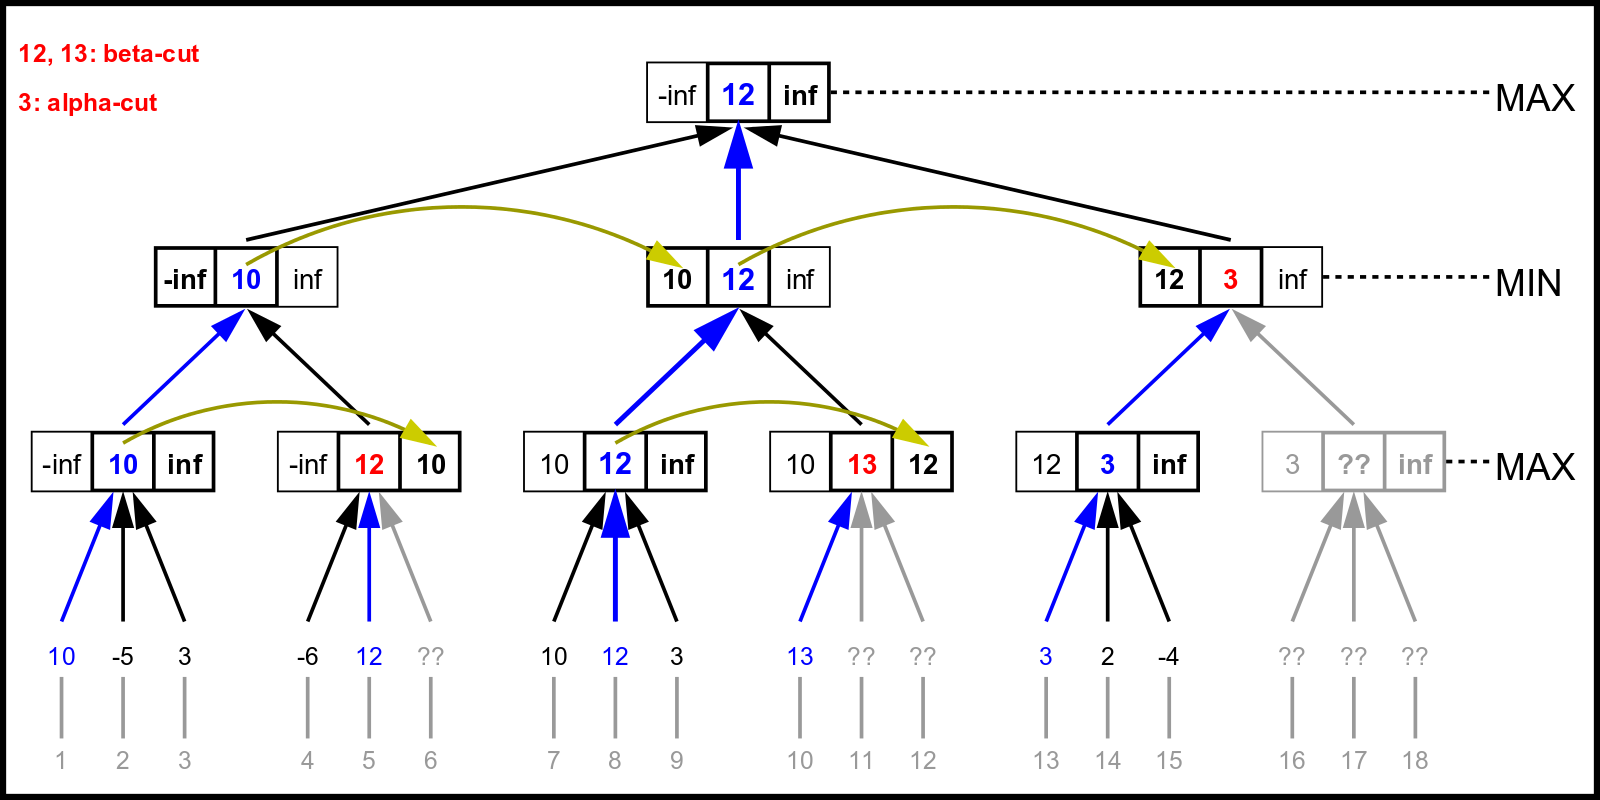
\includegraphics[width=\linewidth]{alphabetawiki.png}
\footnote{\tiny Von de:Benutzer:Antonsusi, using a PNG from Benutzer:Sgop - selbst erstellt/gezeichnet, \textbf{Gemeinfrei}, https://commons.wikimedia.org/w/index.php?curid=53982955}
\end{figure}
\end{frame}

\begin{frame}{AI}
\begin{figure}
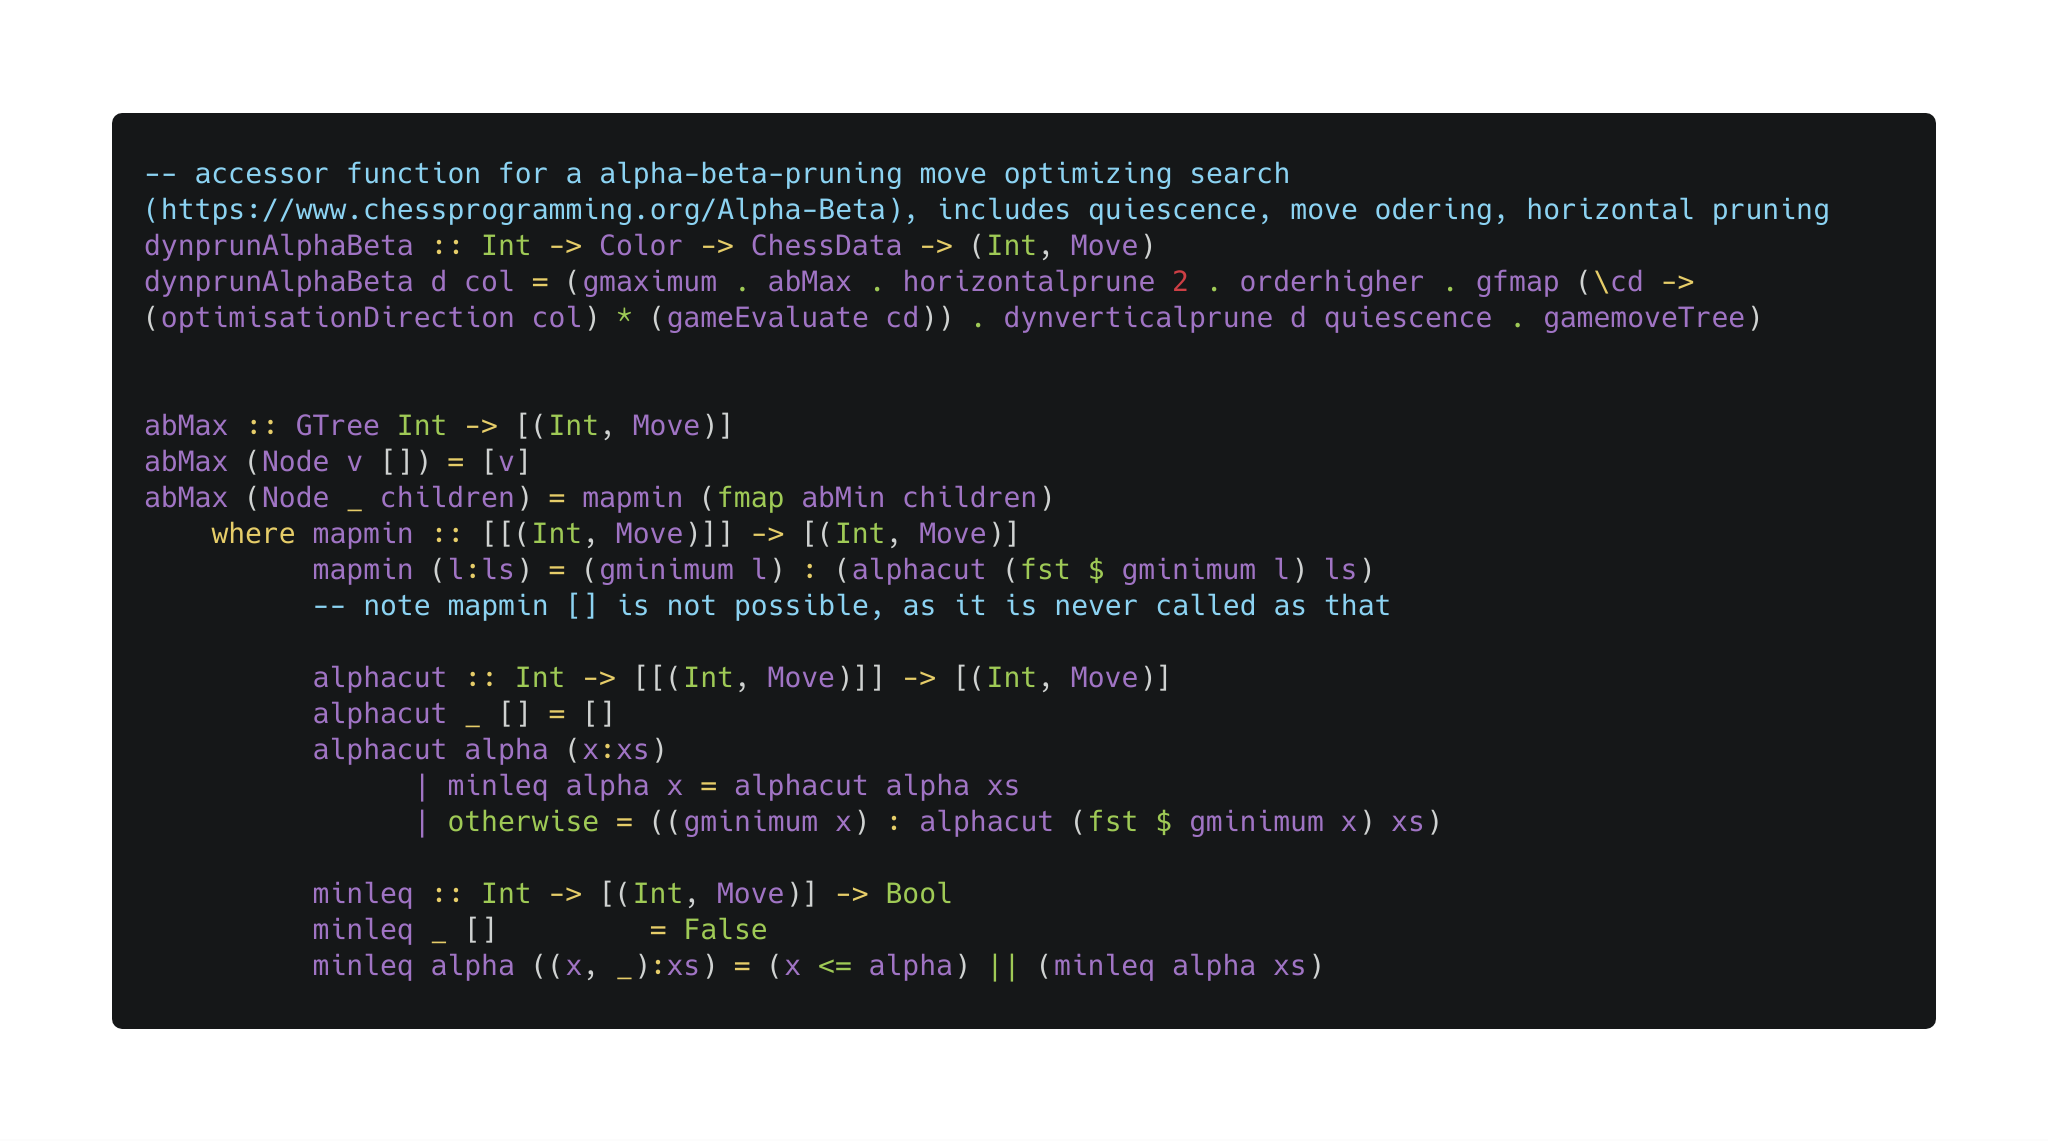
\includegraphics[width=\linewidth]{alphabeta}
\end{figure}
\end{frame}

\begin{frame}{AI}
\begin{figure}
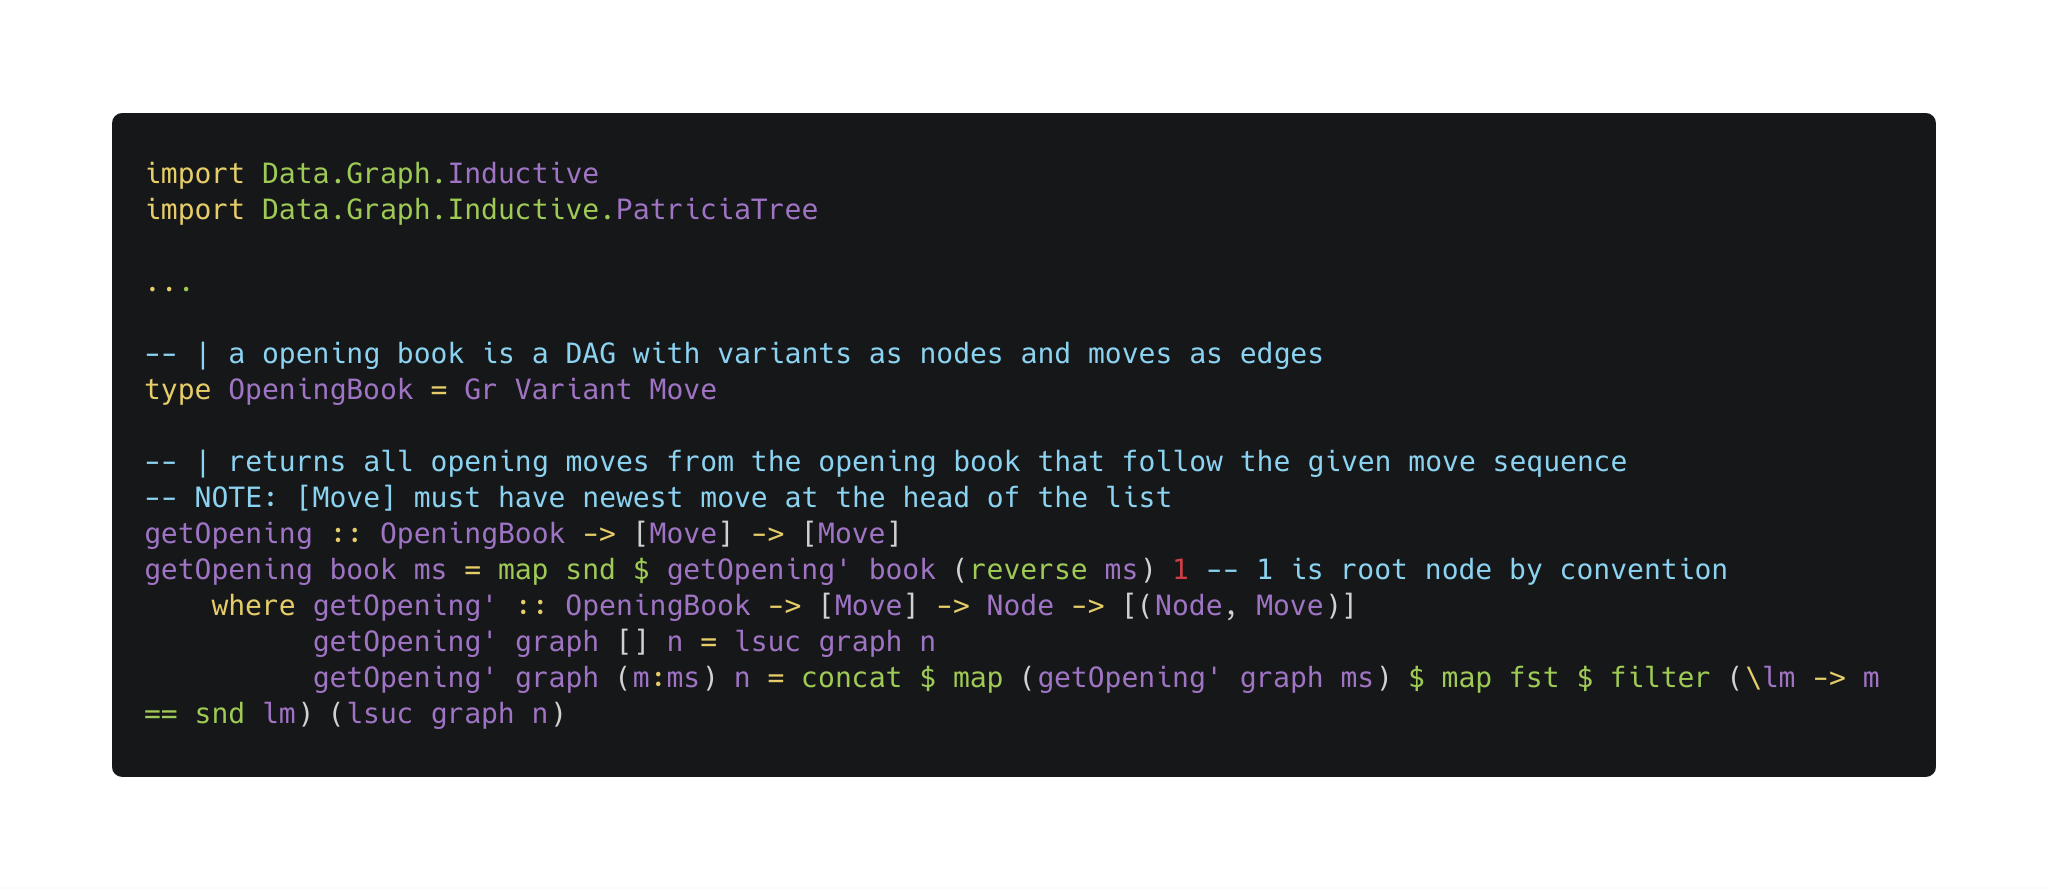
\includegraphics[width=\linewidth]{openingbook.png}
\end{figure}
\end{frame}

\begin{frame}

\begin{columns}

\column{0.5\textwidth}
{\Large \textbf{Render}}

\begin{itemize}
    \item Yesod
\end{itemize}

\column{0.5\textwidth}
\begin{figure}
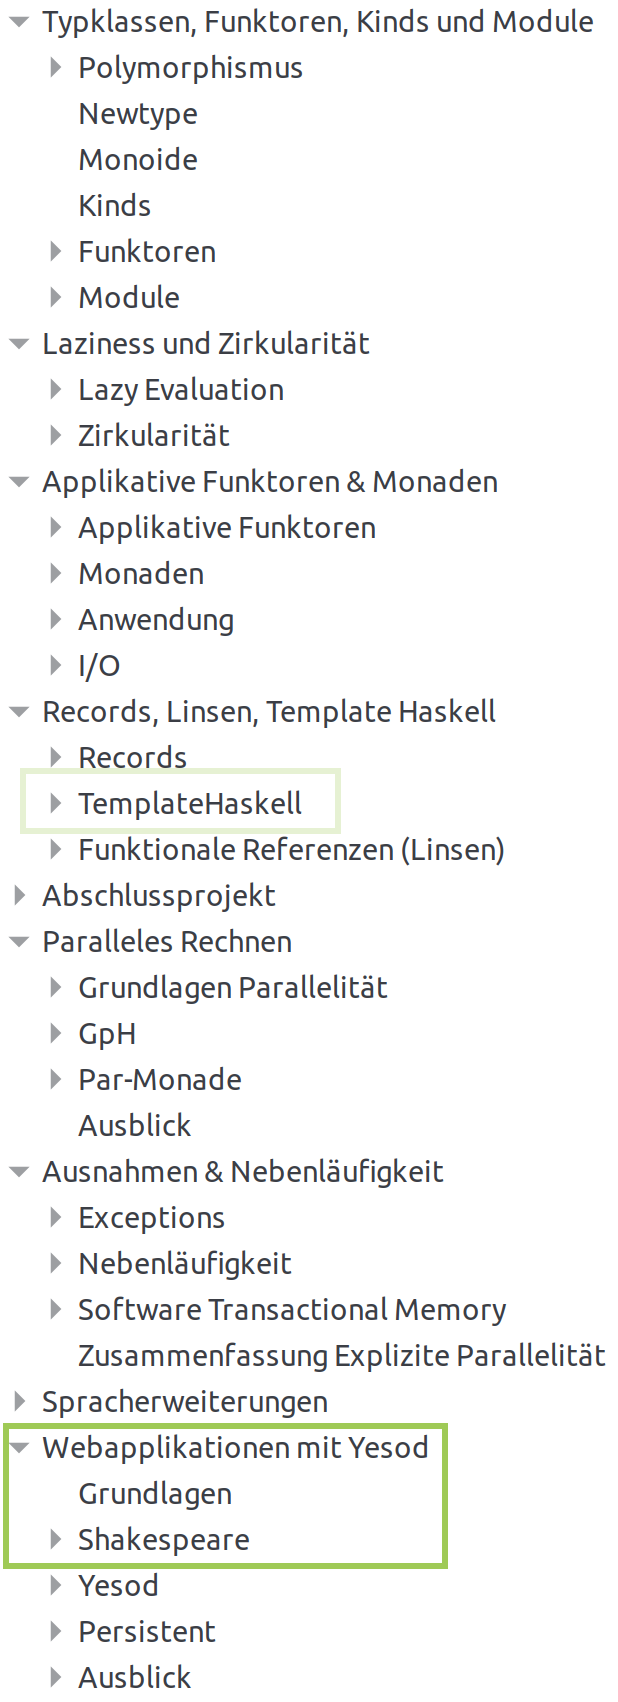
\includegraphics[height=0.9\paperheight]{cont/ssrender.png}
\end{figure}

\end{columns}

\end{frame}

\begin{frame}{Render}
\begin{figure}
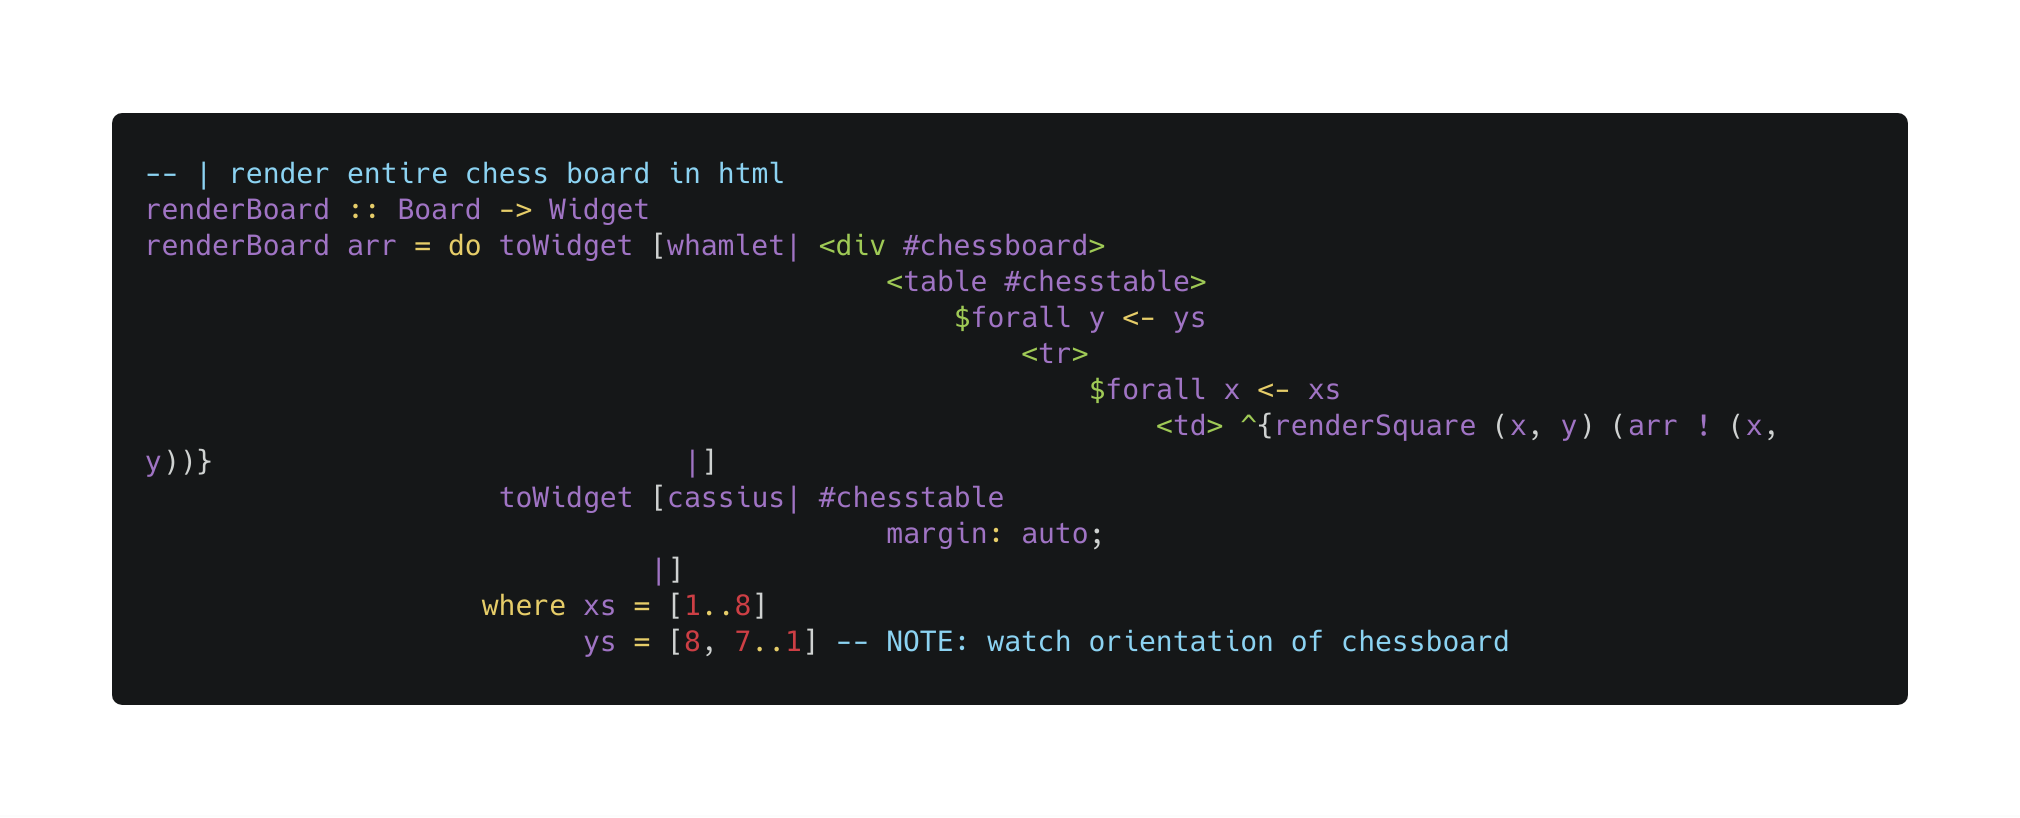
\includegraphics[width=\linewidth]{renderboard}
\end{figure}
\end{frame}



\begin{frame}

\begin{columns}

\column{0.5\textwidth}
{\Large \textbf{Handler - Lobby}}

\begin{itemize}
    \item Yesod
    \item Data.Set
    \item Control.Monad.STM
\end{itemize}


\column{0.5\textwidth}
\begin{figure}
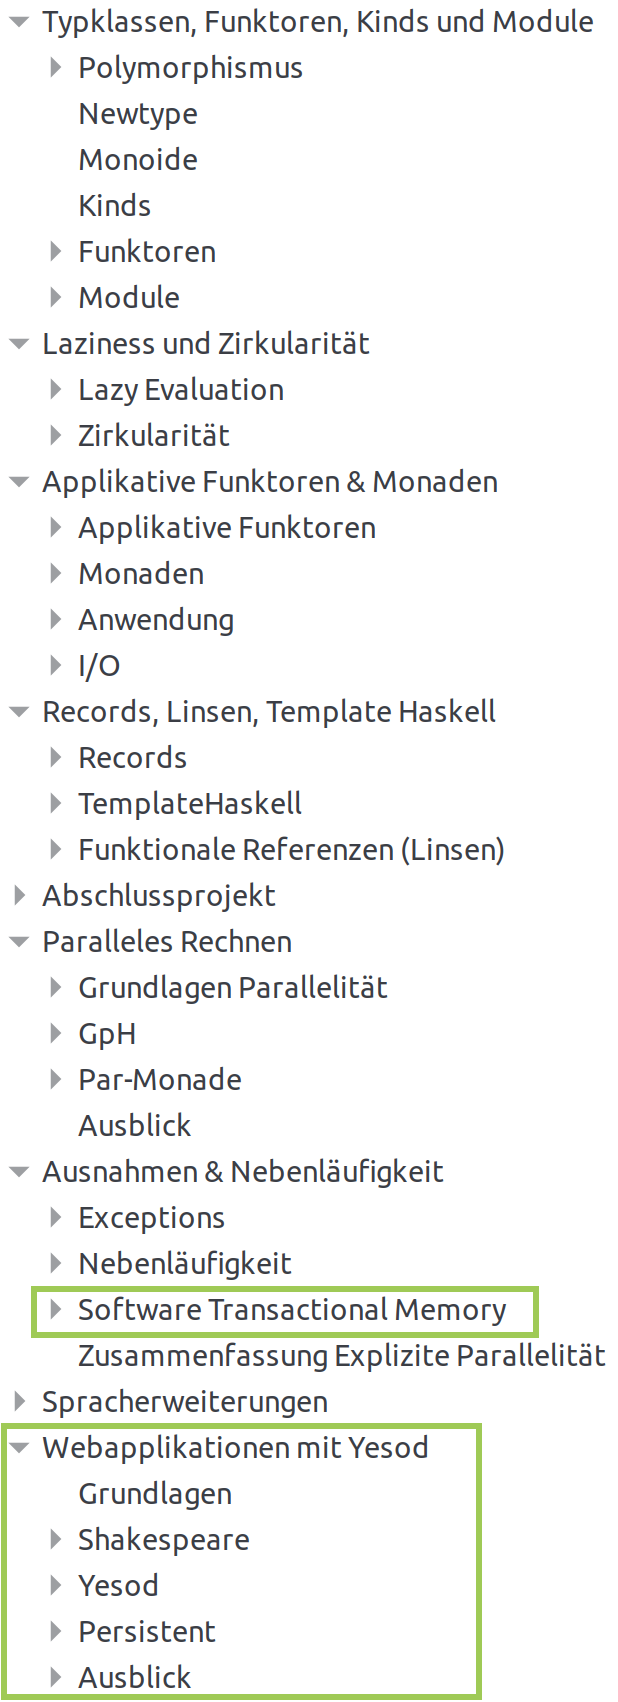
\includegraphics[height=0.9\paperheight]{cont/sslobby.png}
\end{figure}

\end{columns}

\end{frame}

\begin{frame}{Handler}
\begin{figure}
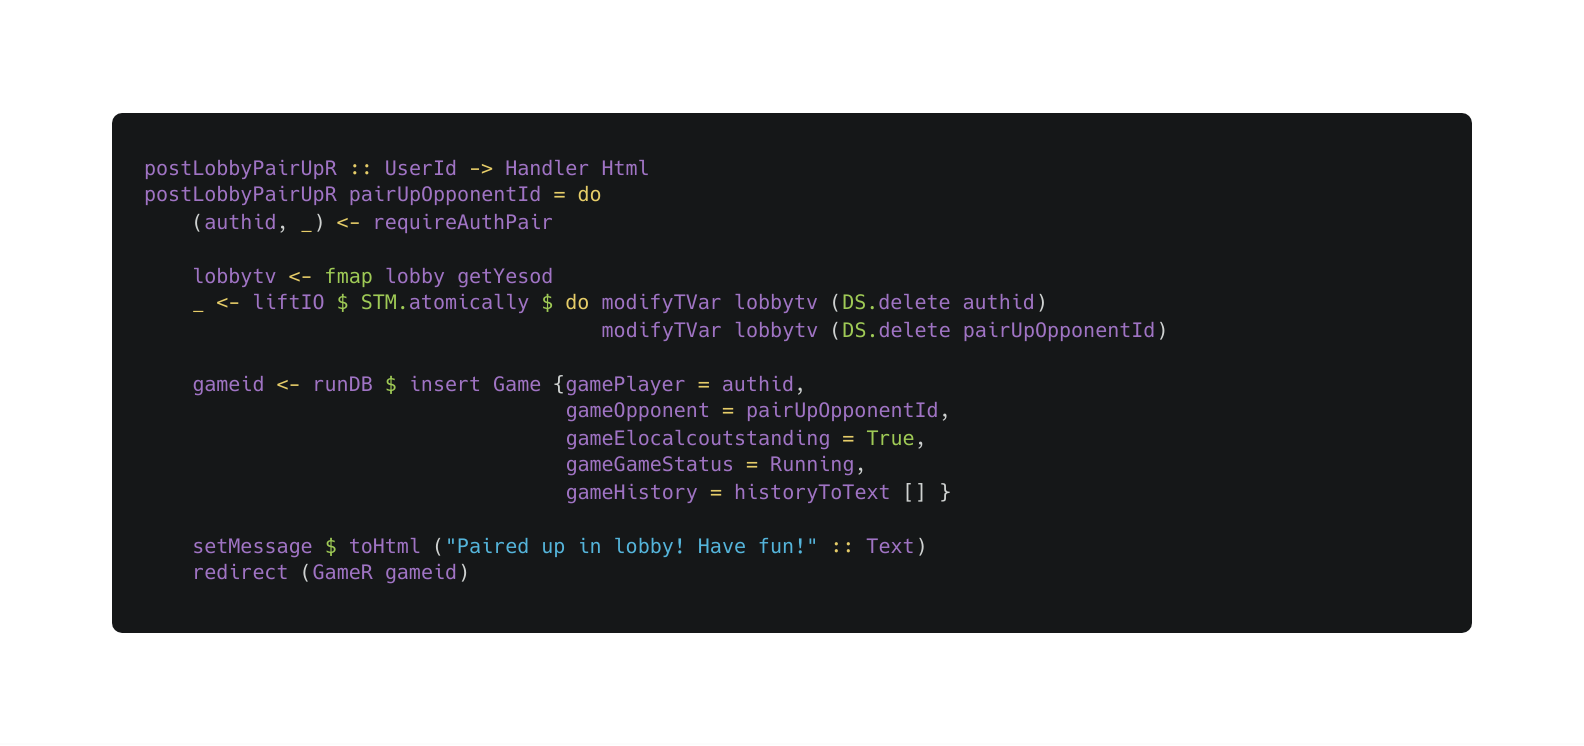
\includegraphics[width=\linewidth]{lobby}
\end{figure}
\end{frame}


\begin{frame}

\begin{columns}

\column{0.5\textwidth}
{\Large \textbf{Handler - AI}}

\begin{itemize}
    \item Yesod
    \item Control.Concurrent
\end{itemize}


\column{0.5\textwidth}
\begin{figure}
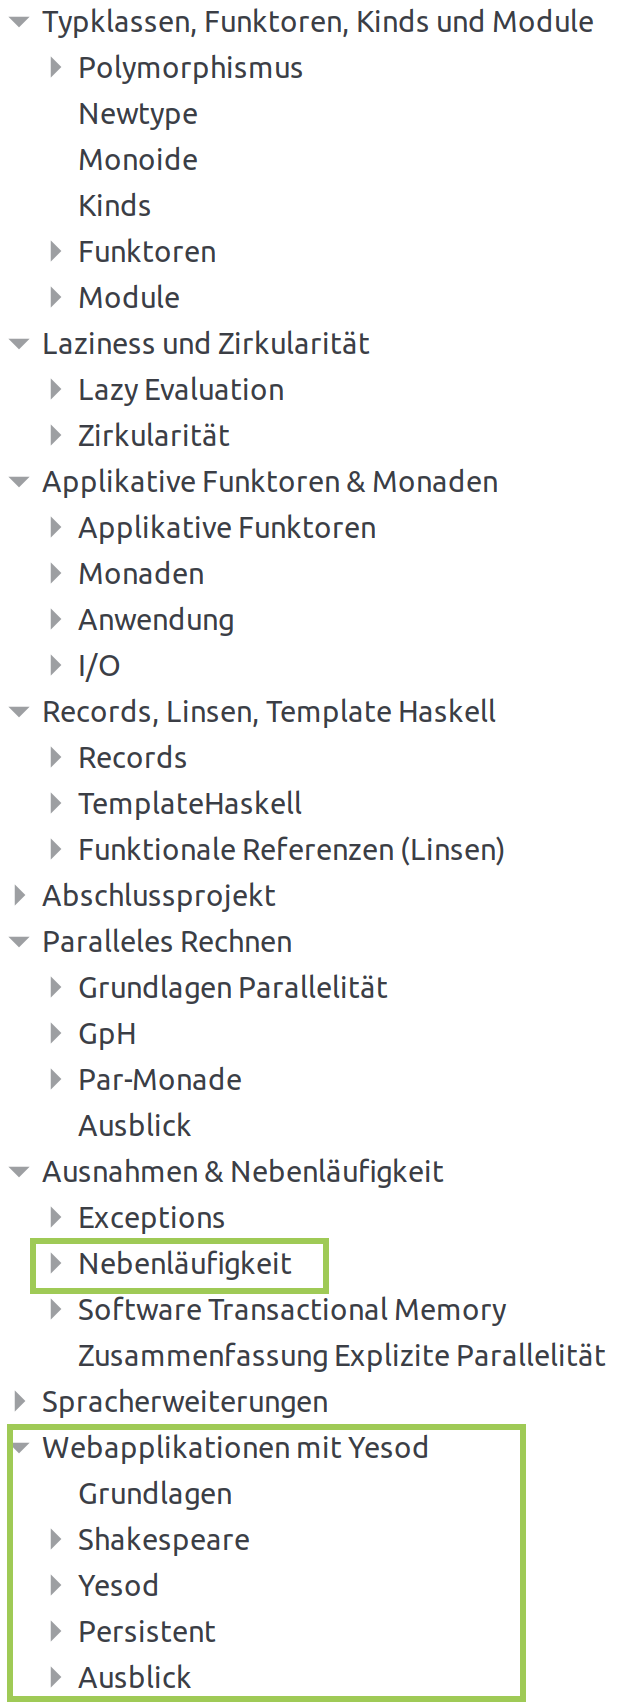
\includegraphics[height=0.9\paperheight]{cont/ssaihandler.png}
\end{figure}

\end{columns}

\end{frame}

\begin{frame}{Handler}
\begin{figure}
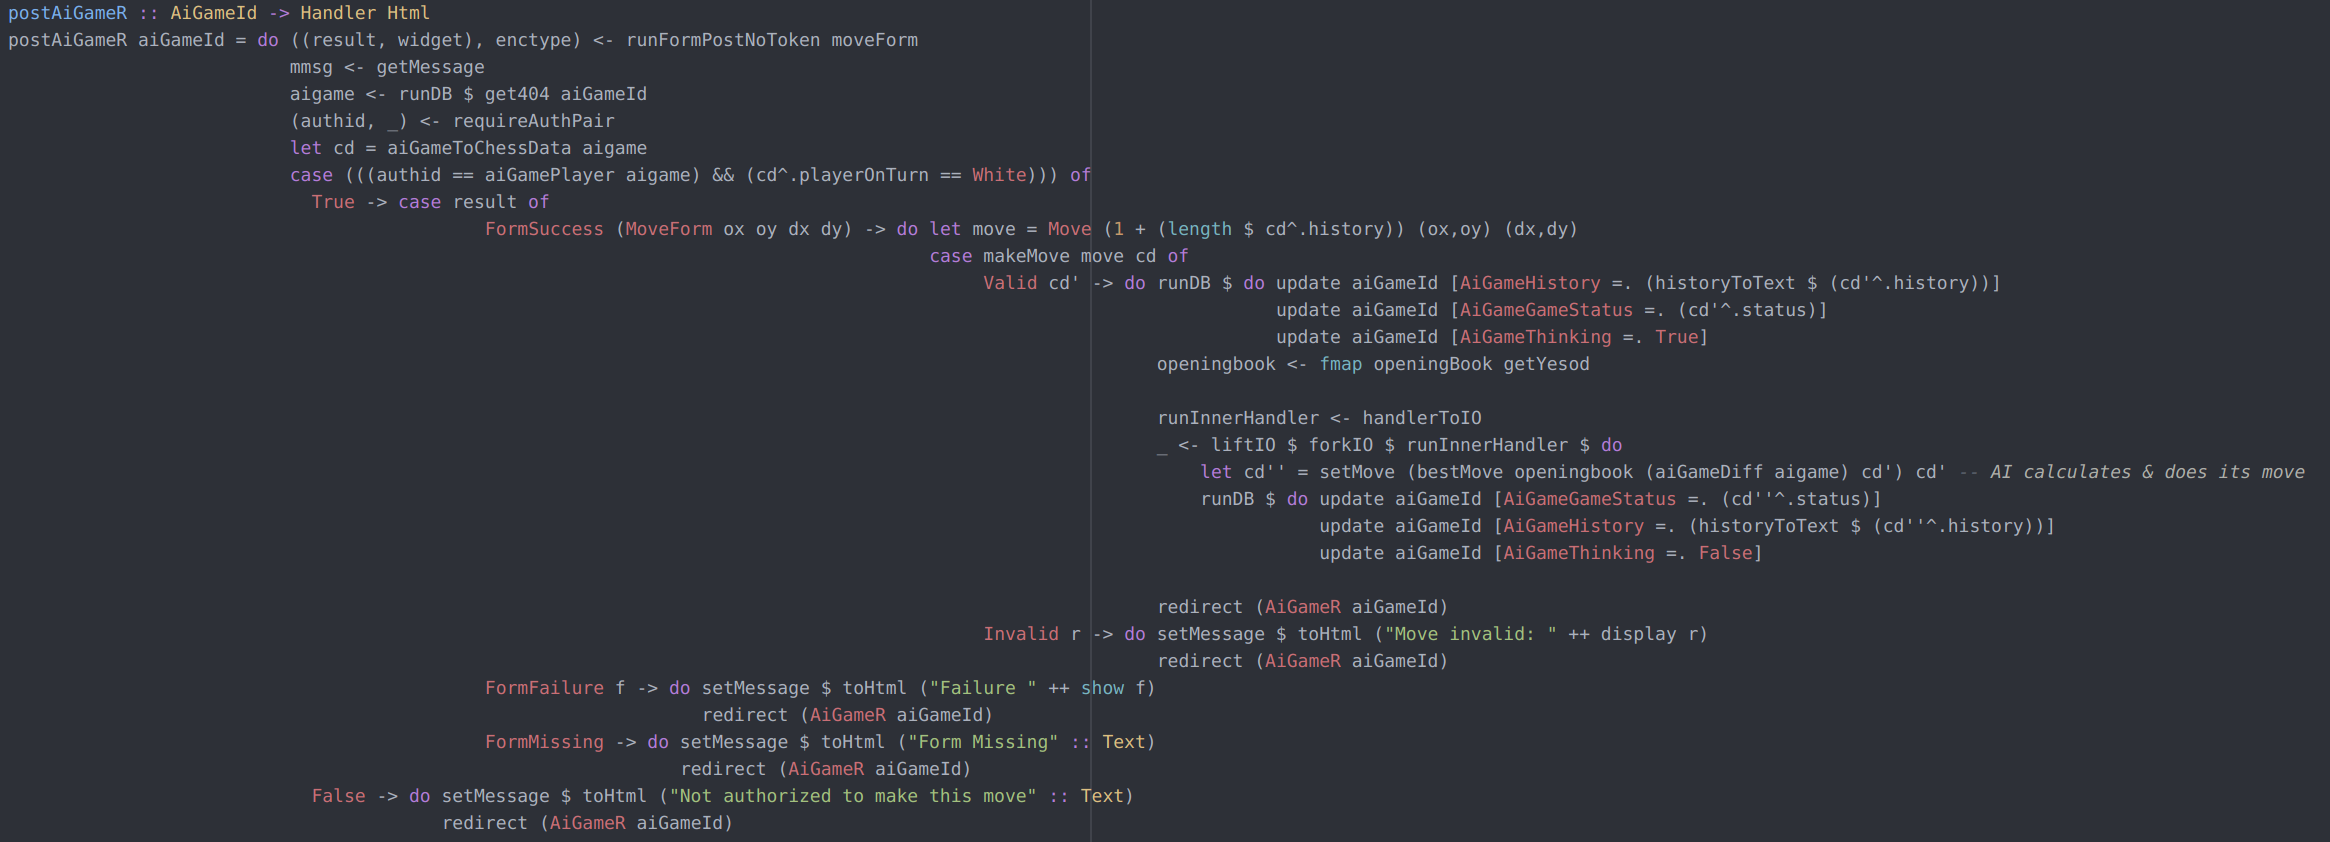
\includegraphics[width=\linewidth]{aihandler}
\end{figure}
\end{frame}

\begin{frame}[plain,c]
\begin{center}
\Huge Danke f\"ur die Aufmerksamkeit!
\end{center}
\end{frame}

\end{document}
